\documentclass[oneside,11pt]{paper}
\usepackage{amsfonts}
\usepackage{amsmath}
\usepackage{mathtools}
\usepackage{tikz}
\usepackage{pgfplotstable}
\usepackage{graphicx}

\graphicspath{{/idiap/user/akomaty/mfGn_results/mfGn-MEMD-codes/Results/}}

\begin{document}

\title{Filter-Bank Structure of Multivariate EMD in multivariate Fractional Gaussian Noise}

\author{A. Komaty and A.O. Boudraa}

\maketitle

\section{Simulations Setup}

We used Wood$\&$Chan's algorithm to simulate multivariate fractional Gaussian noise (mfGn)~\cite{Amblard2010}. The resulting mfGn has the following:
\begin{itemize}
\item The number of channels is $p=8$
\item The correlation parameters used are $\rho \in \{0, 0.2, 0.5, 0.8 \}$
\item The Hurst exponent $H$ takes all values in $\{ 0.2 0.4 0.6 0.8 \}$. It should be noted that when $H=0.5$, the fGn reduces to white Gaussian noise, a topic that was already studied in~\cite{Rehman2011}.
\item the number of samples for each process is set to $1000$.
\item The number of Monte Carlo (MC) simulations is set to $5000$ in order to be as precise as possible with average results.
\item Because the number of obtained IMFs differs from simulation to another, we decided to keep the first $8$ IMFs for all simulations.
\end{itemize}

\section{IMFs Power-Spectra}
In figure~\ref{fig:Power_Spectra_MEMD}, we show the power spectrum of the obtained IMFs for different parameter combination $(\rho, H)$. These results are the mean over $5000$ MC runs. Figure~\ref{fig:Normalized_Power_Spectra_MEMD} shows the normalized power spectrum, the normalisation is performed according to the following equation:
\begin{equation}
S_{m,p,H}(f)=\rho_H^{a(m-l)} S_{l,p,H}(\rho_H^{m-l} f)
\label{eq: S_k_rho}
\end{equation}

\begin{figure}[htbp]
\hspace{-2cm}
\begin{tabular}{c c c c}
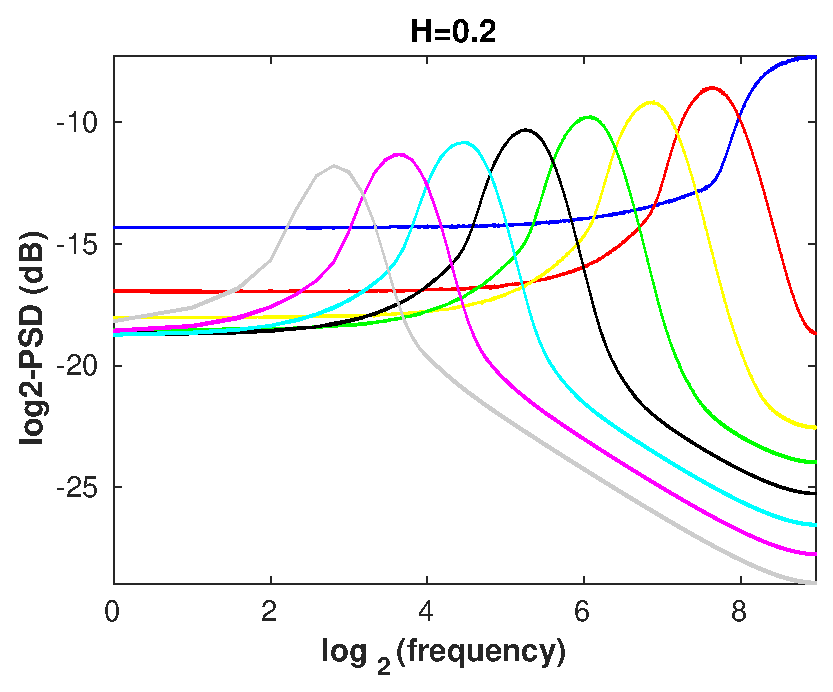
\includegraphics[scale=0.27]{SPEC_NDel_0_H_2.eps}&
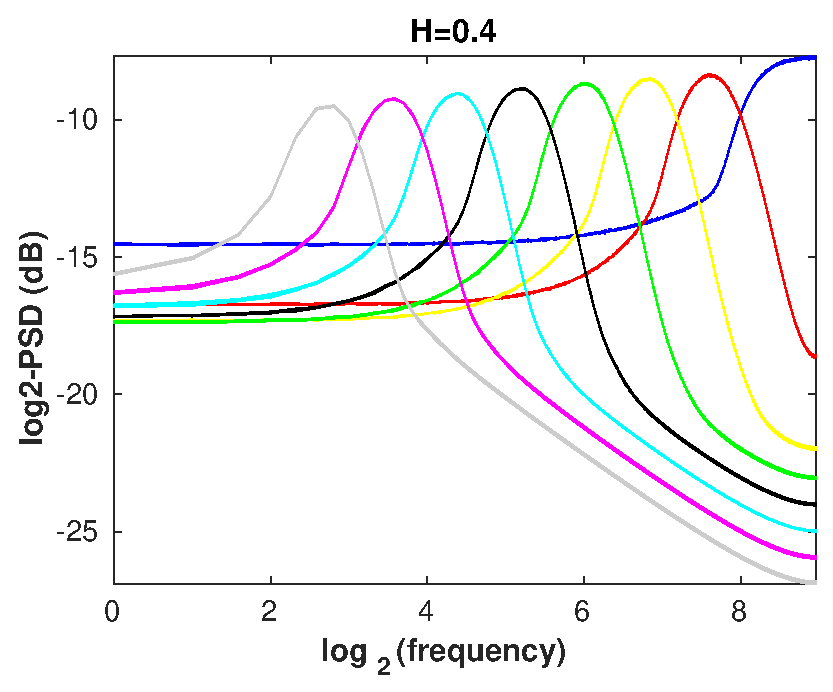
\includegraphics[scale=0.27]{SPEC_NDel_0_H_4.eps}&
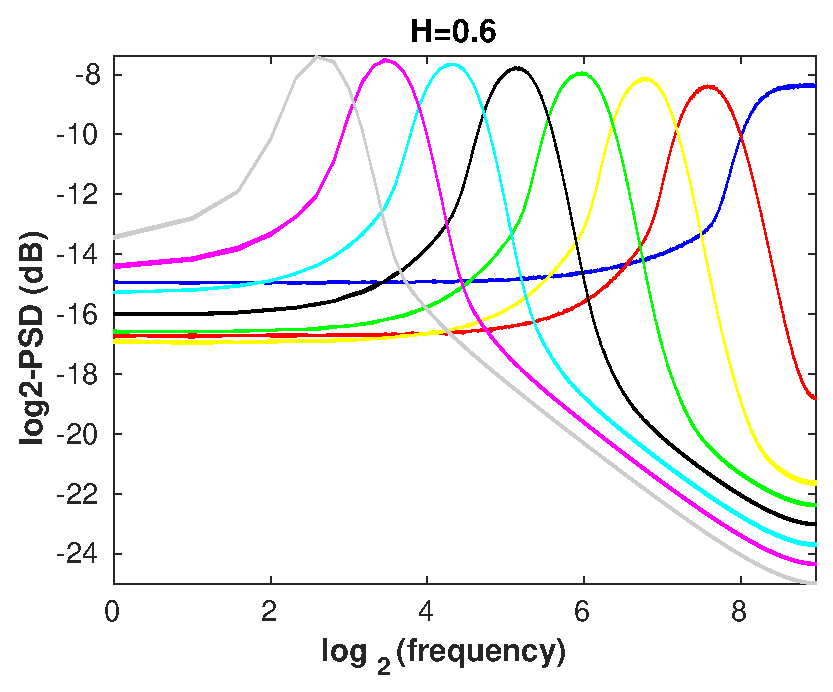
\includegraphics[scale=0.27]{SPEC_NDel_0_H_6.eps}&
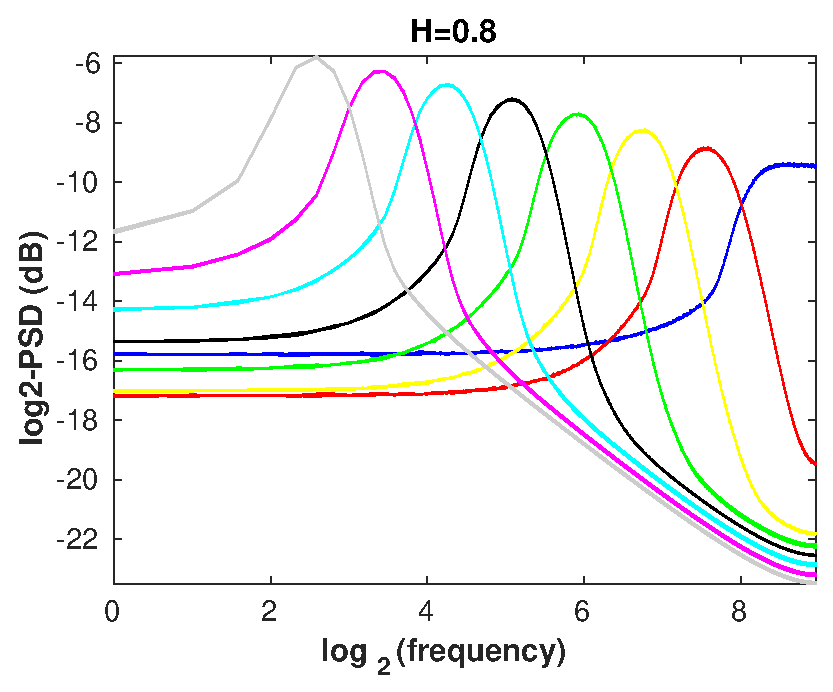
\includegraphics[scale=0.27]{SPEC_NDel_0_H_8.eps}\\
 $\rho=0,~H=0.2$ & $\rho=0,~H=0.4$ & $\rho=0,~H=0.6$ & $\rho=0,~H=0.8$\\
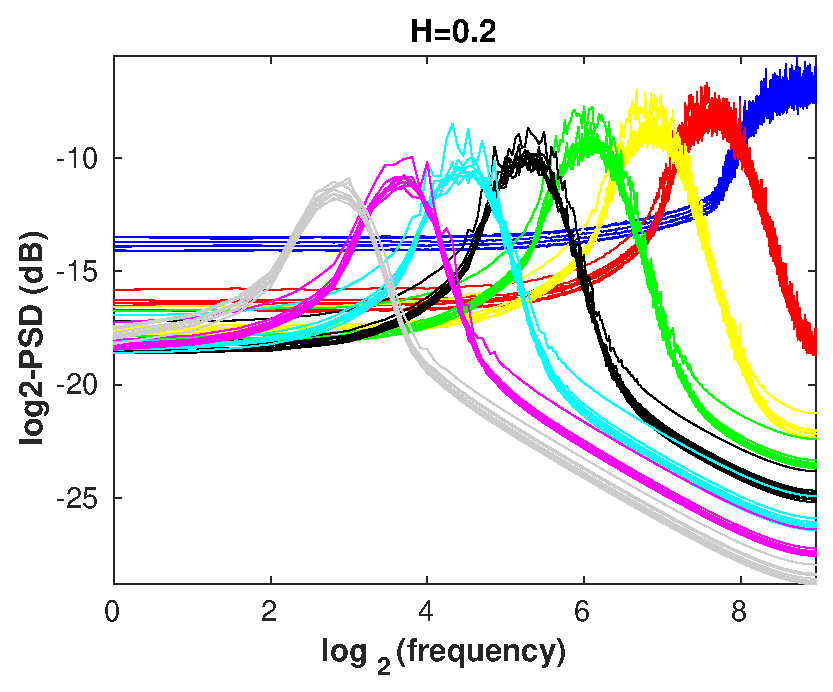
\includegraphics[scale=0.27]{SPEC_NDel_2_H_2.eps}&
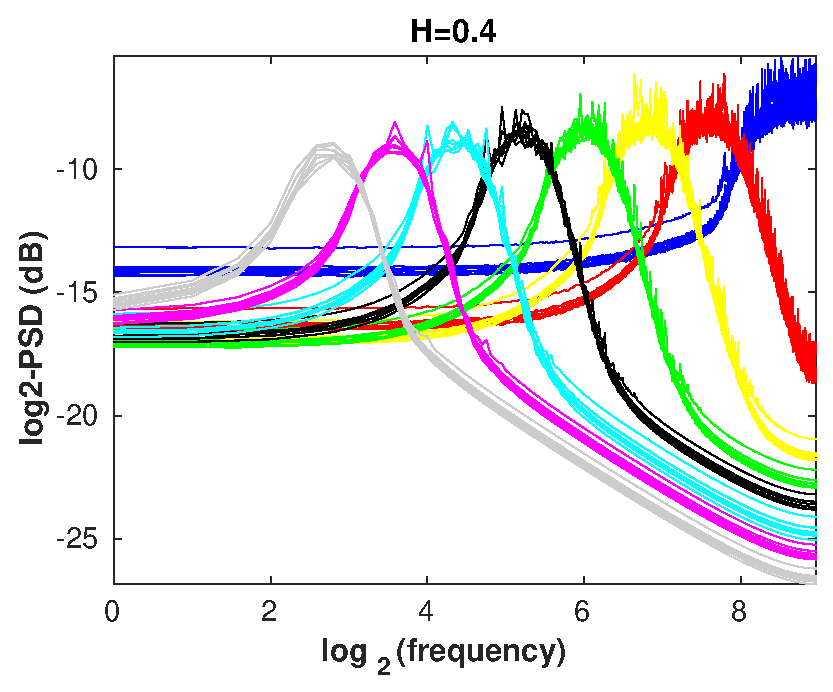
\includegraphics[scale=0.27]{SPEC_NDel_2_H_4.eps}&
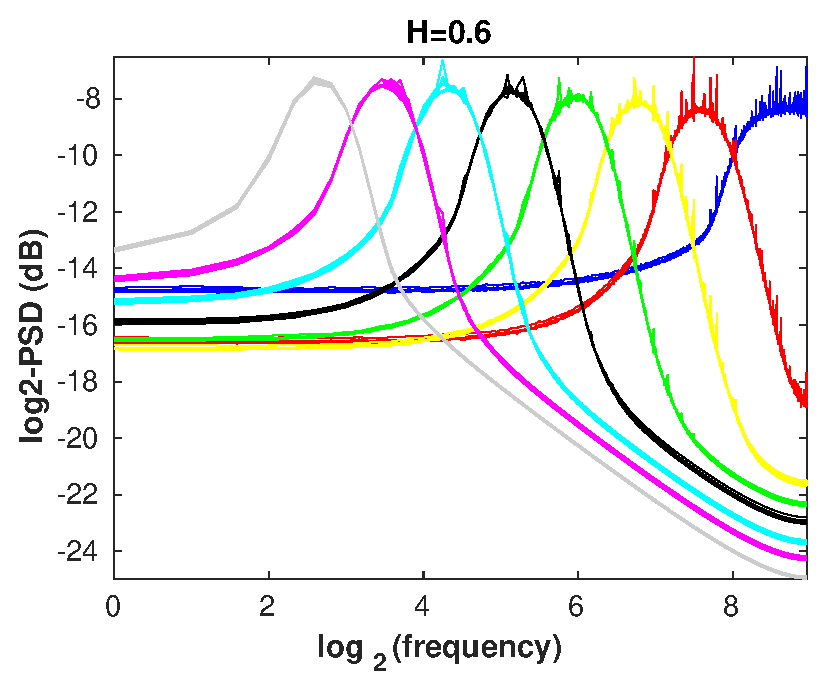
\includegraphics[scale=0.27]{SPEC_NDel_2_H_6.eps}&
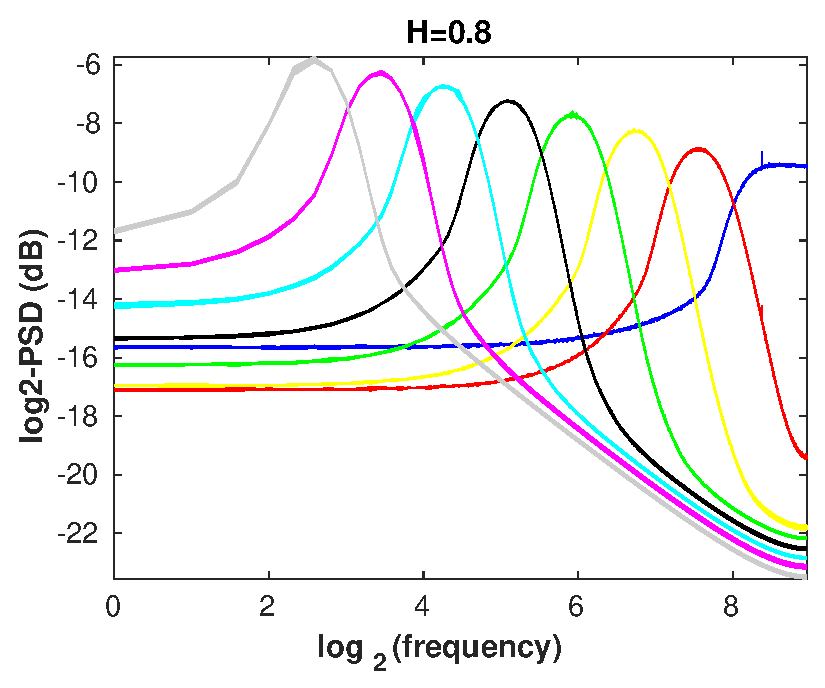
\includegraphics[scale=0.27]{SPEC_NDel_2_H_8.eps}\\
 $\rho=0.2,~H=0.2$ & $\rho=0.2,~H=0.4$ & $\rho=0.2,~H=0.6$ & $\rho=0.2,~H=0.8$\\
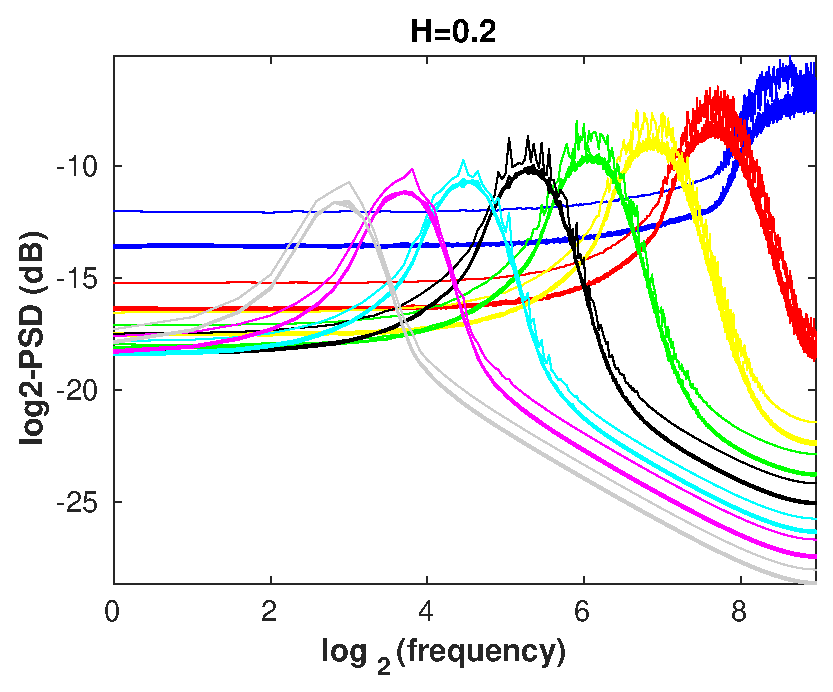
\includegraphics[scale=0.27]{SPEC_NDel_5_H_2.eps}&
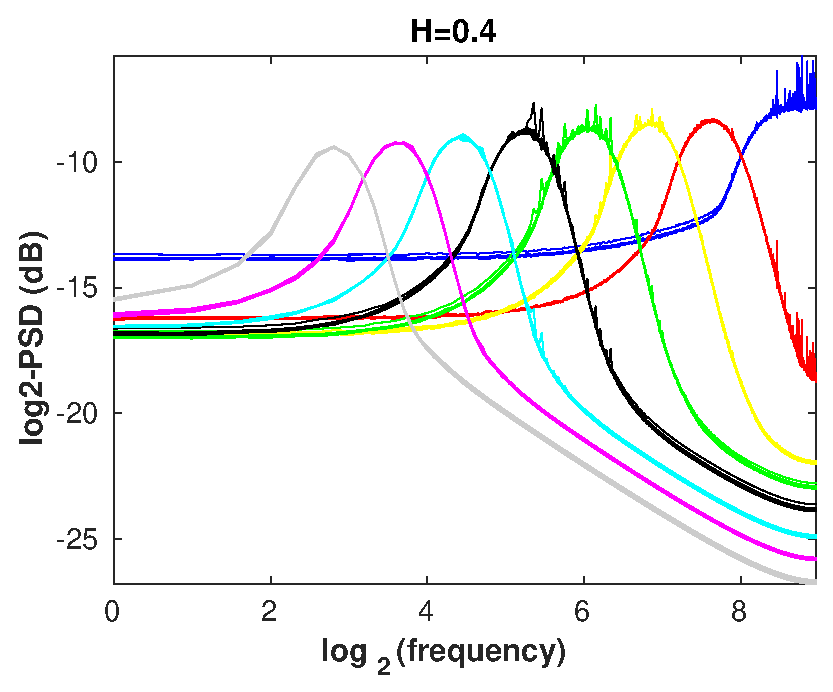
\includegraphics[scale=0.27]{SPEC_NDel_5_H_4.eps}&
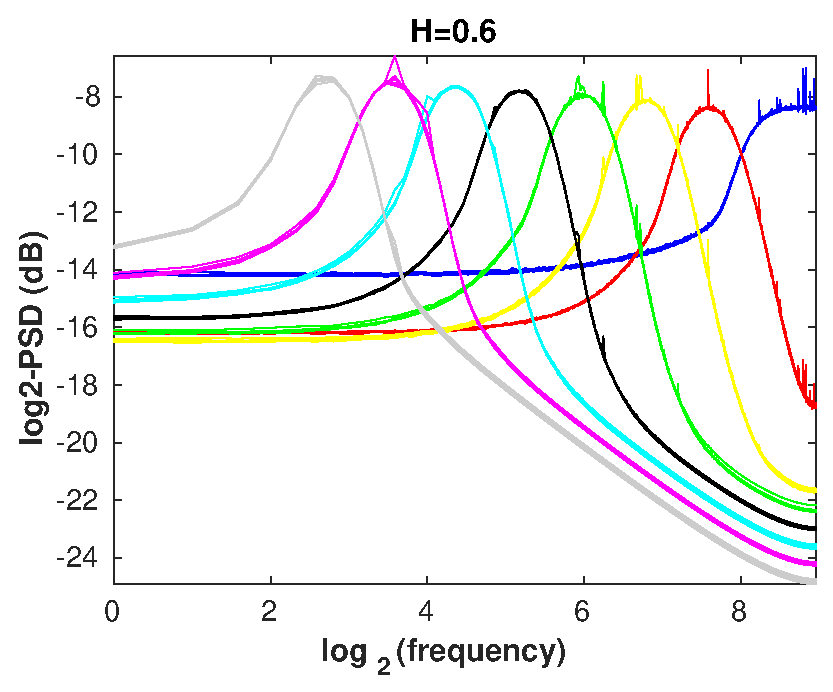
\includegraphics[scale=0.27]{SPEC_NDel_5_H_6.eps}&
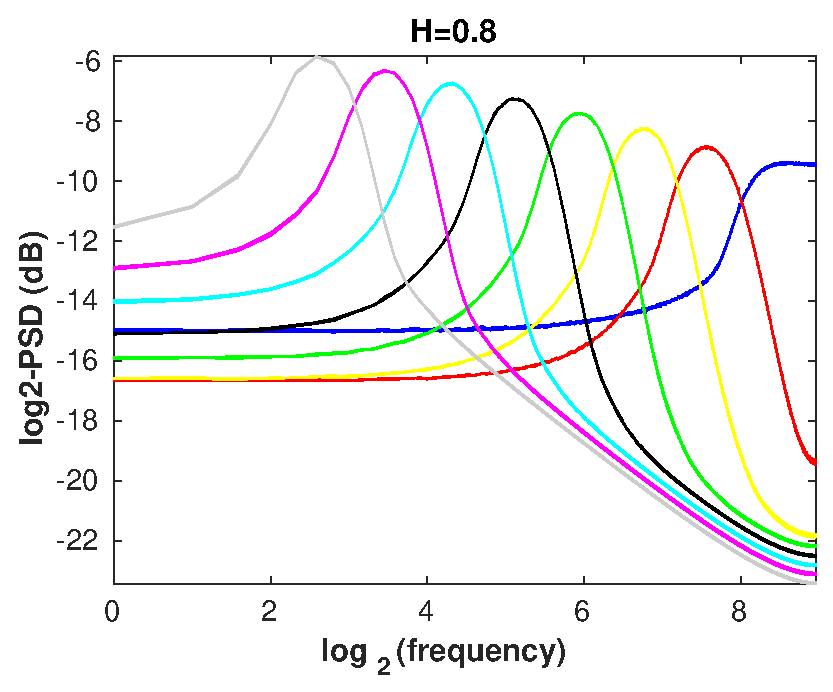
\includegraphics[scale=0.27]{SPEC_NDel_5_H_8.eps}\\
 $\rho=0.5,~H=0.2$ & $\rho=0.5,~H=0.4$ & $\rho=0.5,~H=0.6$ & $\rho=0.5,~H=0.8$\\
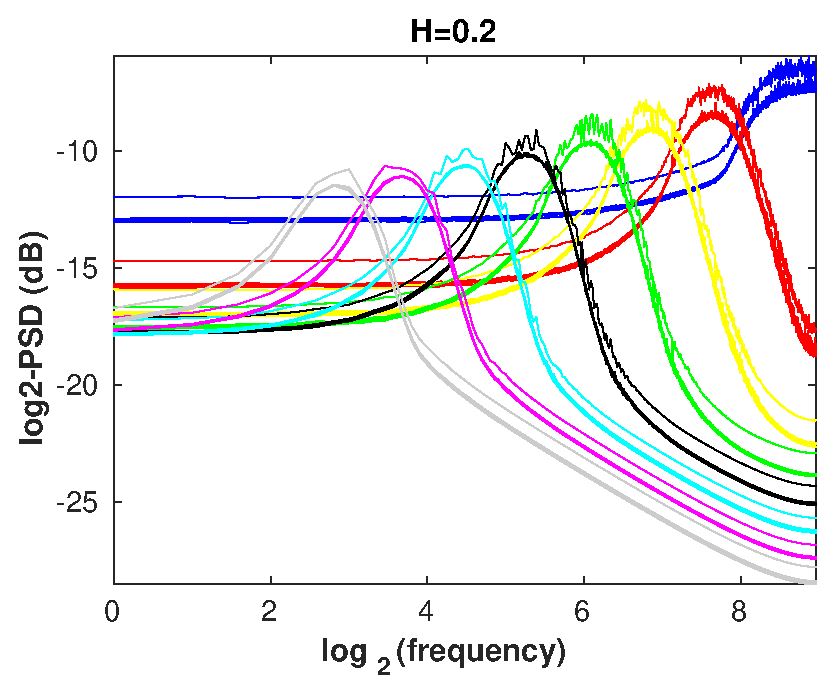
\includegraphics[scale=0.27]{SPEC_NDel_8_H_2.eps}&
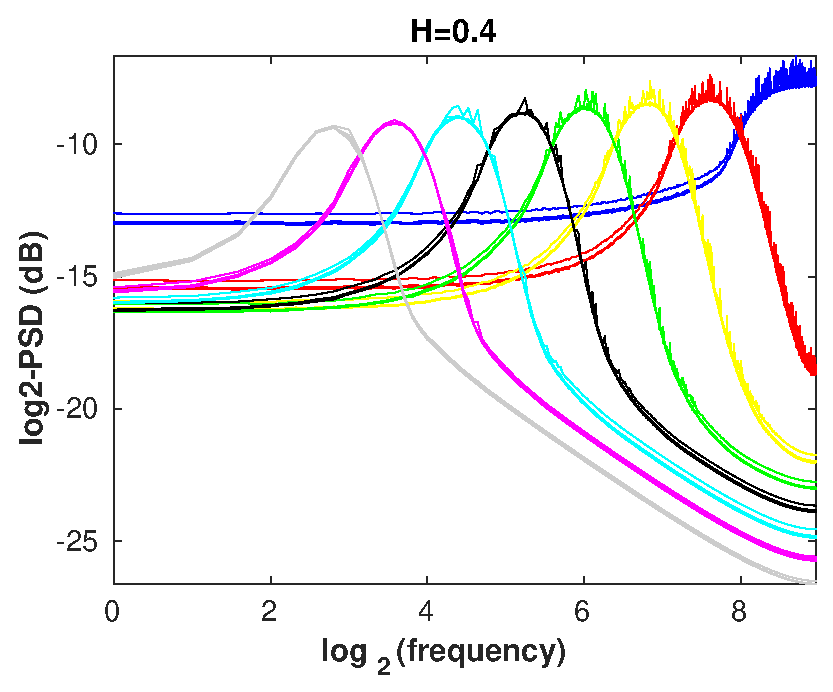
\includegraphics[scale=0.27]{SPEC_NDel_8_H_4.eps}&
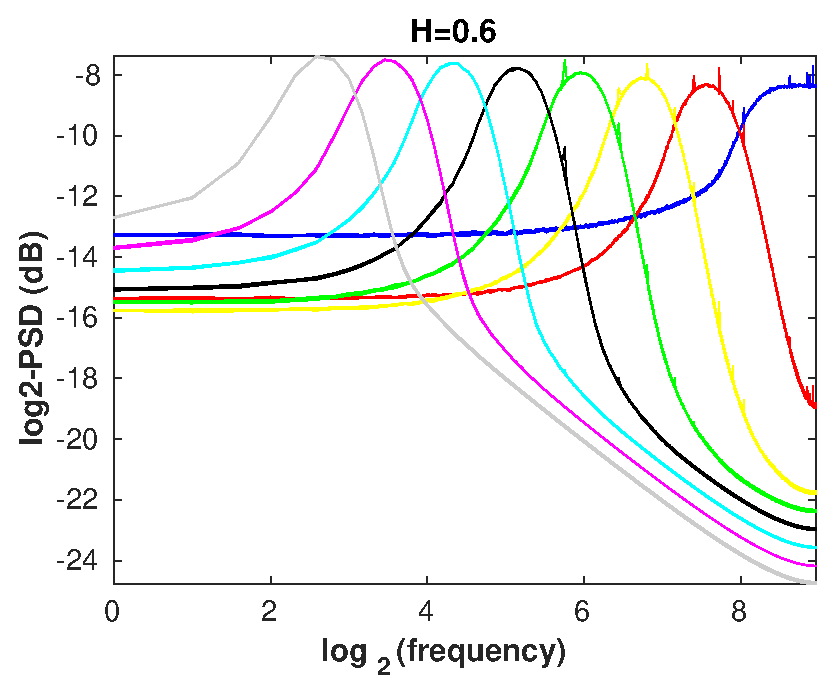
\includegraphics[scale=0.27]{SPEC_NDel_8_H_6.eps}&
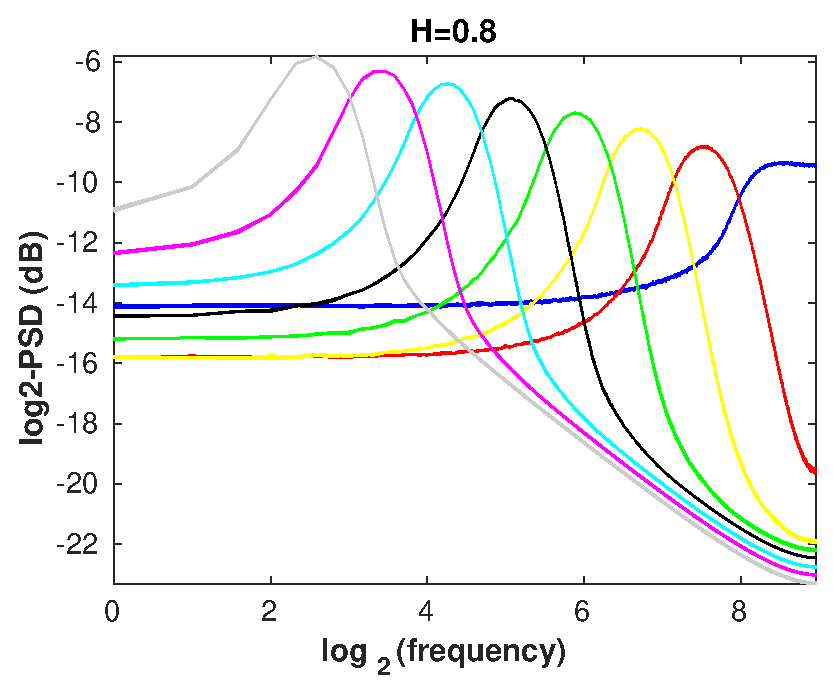
\includegraphics[scale=0.27]{SPEC_NDel_8_H_8.eps}\\
 $\rho=0.8,~H=0.2$ & $\rho=0.8,~H=0.4$ & $\rho=0.8,~H=0.6$ & $\rho=0.8,~H=0.8$\\
\end{tabular}
\caption{The power spectra of IMFs as a function of $\log_2(f)$, for $H \in \{0.2,0.4, 0.6, 0.8\}$ and $\rho \in \{0, 0.2,0.5,0.8\}$. Overlapping of the frequency bands corresponds to the same-index IMFs, showing the mode alignment. We notice some leak in some values of $(\rho, H)$, this could be due to the correlation between channels.}
\label{fig:Power_Spectra_MEMD}
\end{figure}


\begin{figure}[htbp]
\hspace{-2cm}
\begin{tabular}{c c c c}
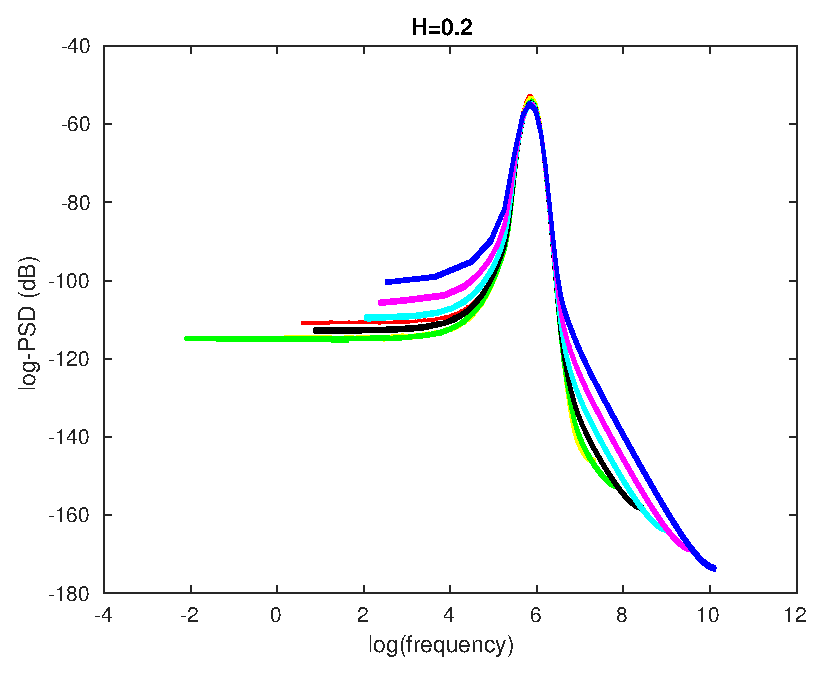
\includegraphics[scale=0.27]{SPEC_Norm_NDel_0_H_2.eps}&
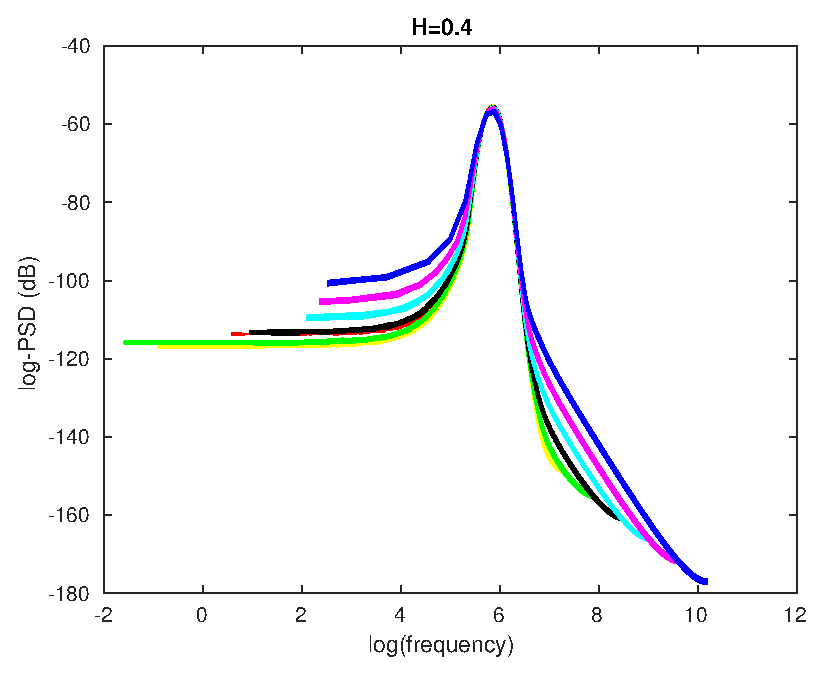
\includegraphics[scale=0.27]{SPEC_Norm_NDel_0_H_4.eps}&
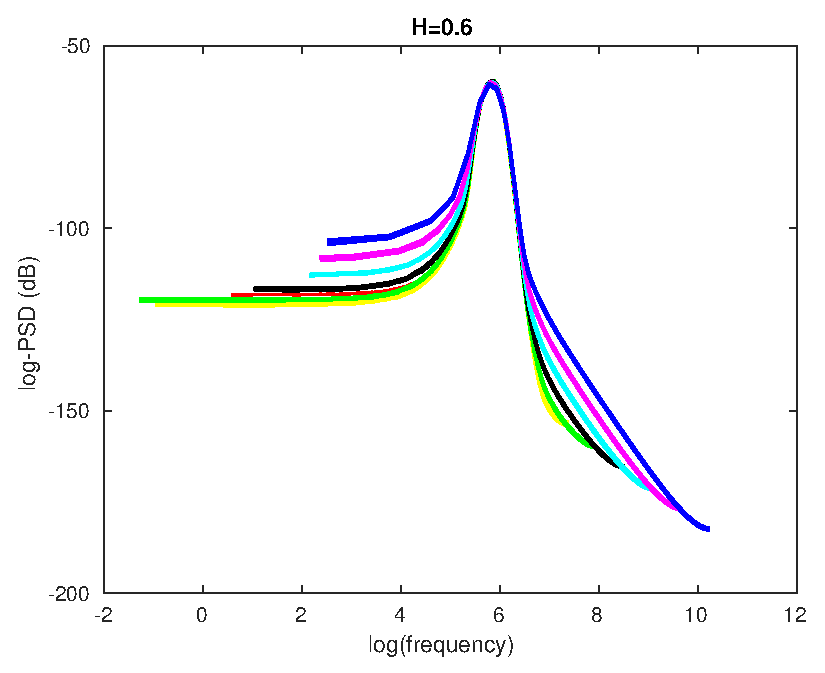
\includegraphics[scale=0.27]{SPEC_Norm_NDel_0_H_6.eps}&
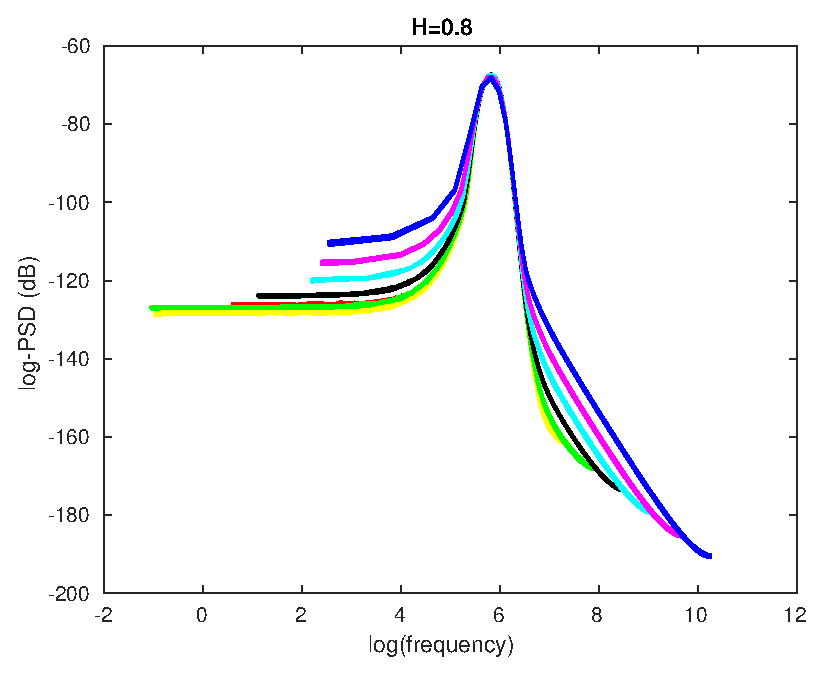
\includegraphics[scale=0.27]{SPEC_Norm_NDel_0_H_8.eps}\\
 $\rho=0,~H=0.2$ & $\rho=0,~H=0.4$ & $\rho=0,~H=0.6$ & $\rho=0,~H=0.8$\\
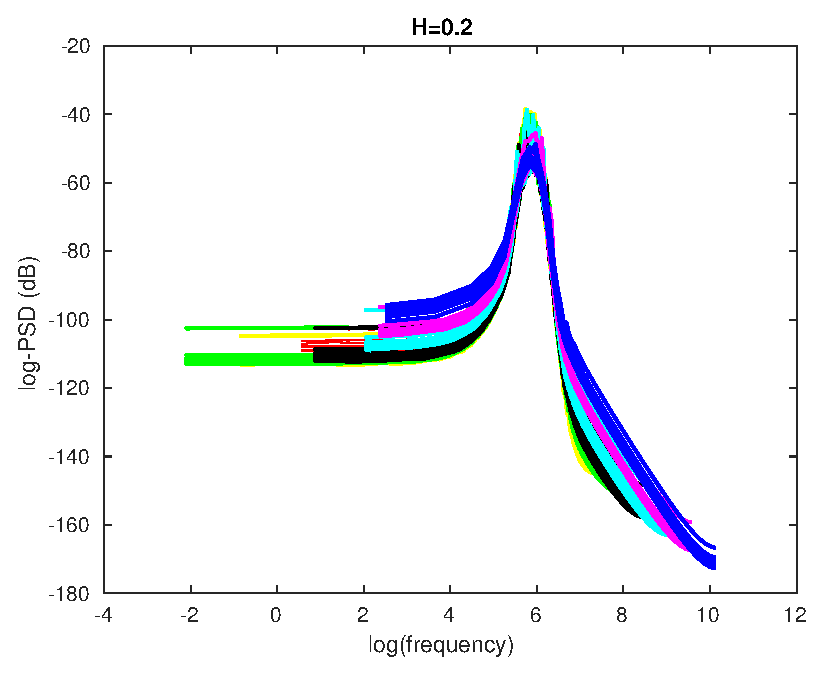
\includegraphics[scale=0.27]{SPEC_Norm_NDel_2_H_2.eps}&
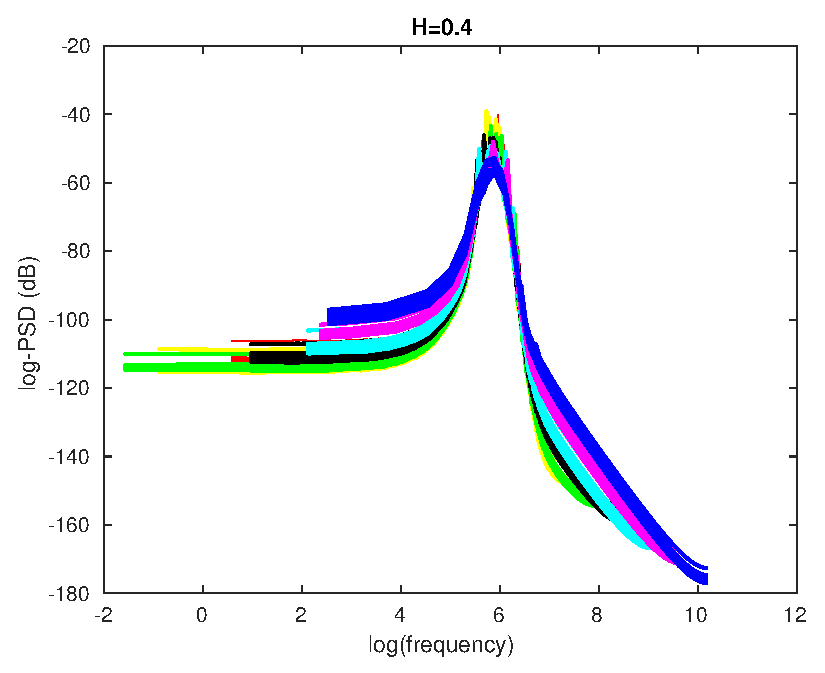
\includegraphics[scale=0.27]{SPEC_Norm_NDel_2_H_4.eps}&
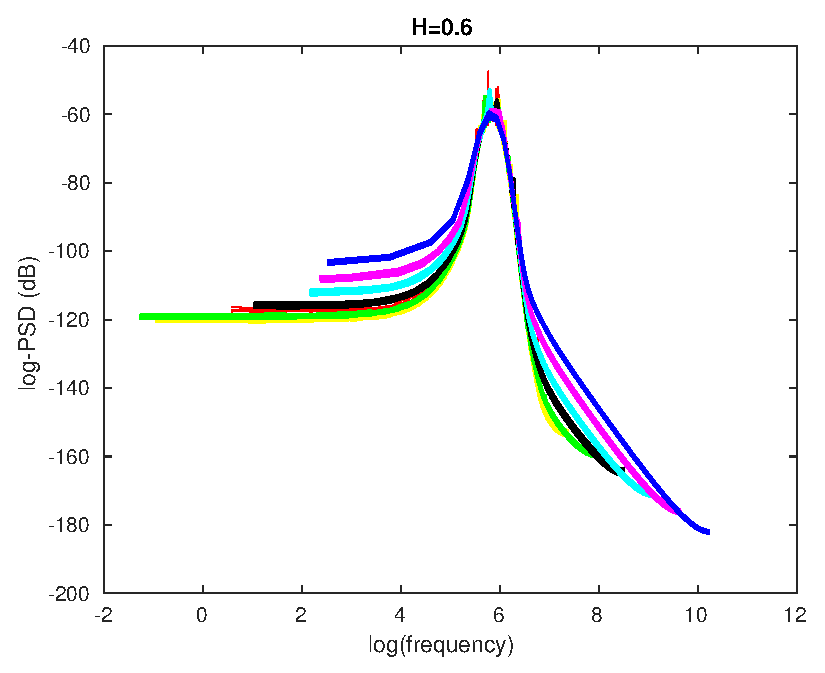
\includegraphics[scale=0.27]{SPEC_Norm_NDel_2_H_6.eps}&
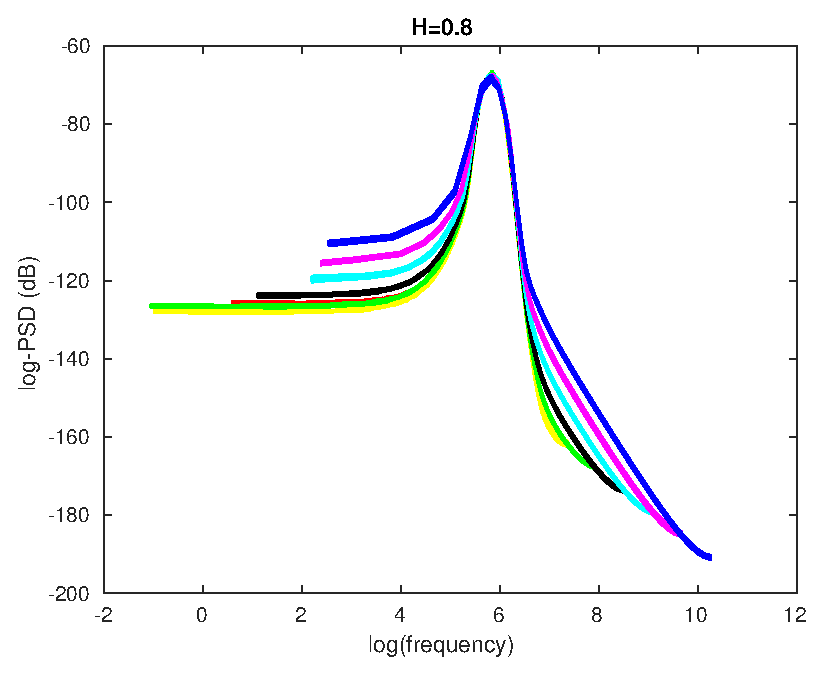
\includegraphics[scale=0.27]{SPEC_Norm_NDel_2_H_8.eps}\\
 $\rho=0.2,~H=0.2$ & $\rho=0.2,~H=0.4$ & $\rho=0.2,~H=0.6$ & $\rho=0.2,~H=0.8$\\
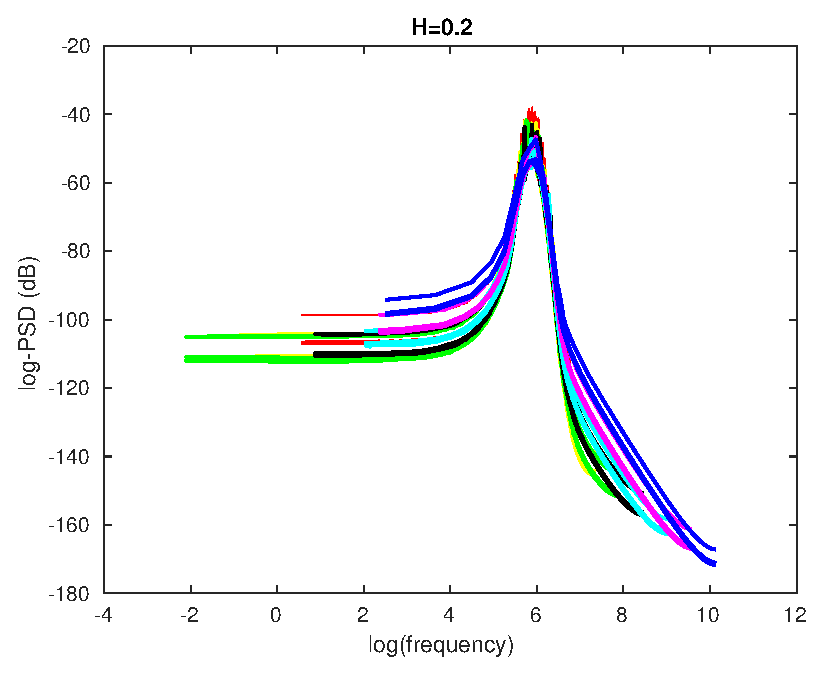
\includegraphics[scale=0.27]{SPEC_Norm_NDel_5_H_2.eps}&
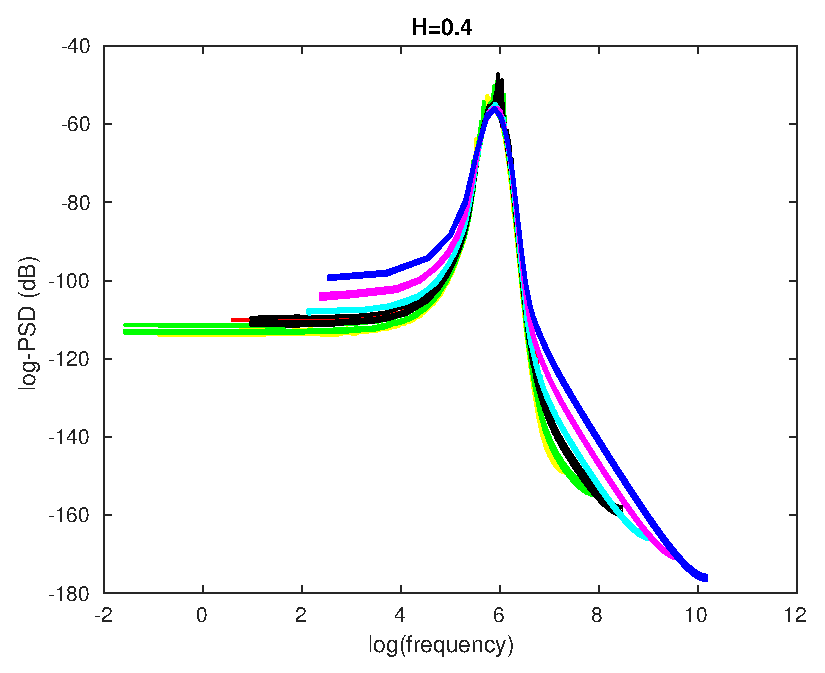
\includegraphics[scale=0.27]{SPEC_Norm_NDel_5_H_4.eps}&
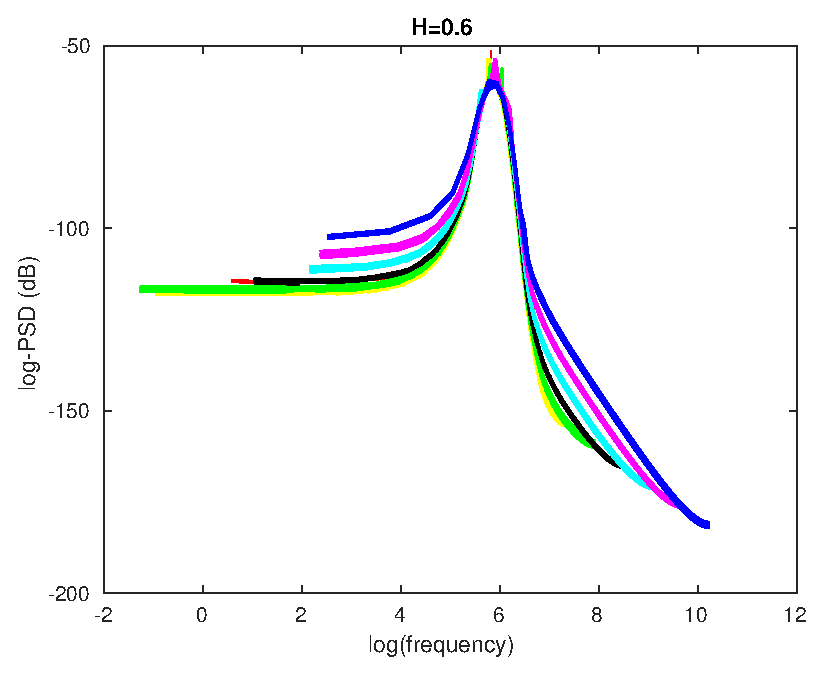
\includegraphics[scale=0.27]{SPEC_Norm_NDel_5_H_6.eps}&
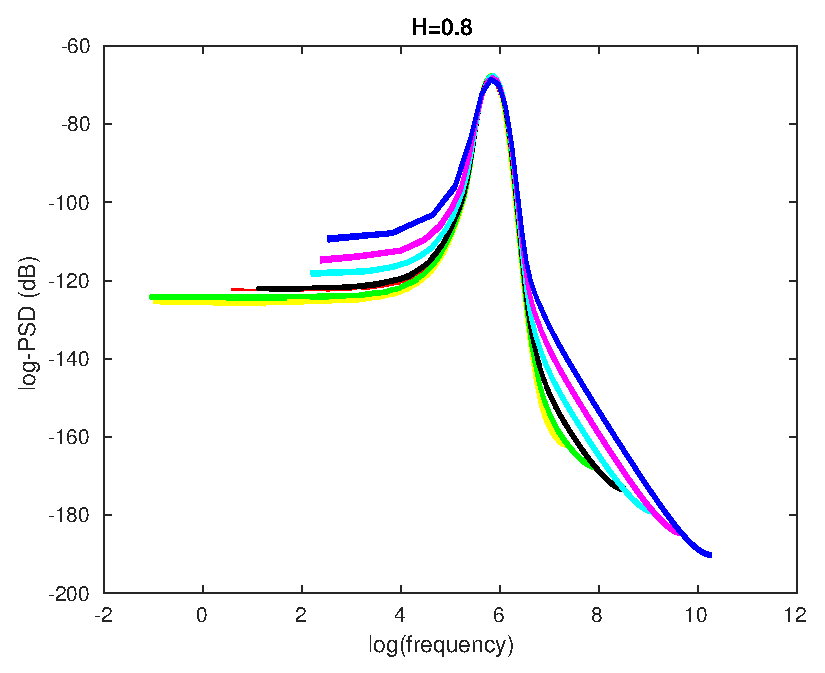
\includegraphics[scale=0.27]{SPEC_Norm_NDel_5_H_8.eps}\\
 $\rho=0.5,~H=0.2$ & $\rho=0.5,~H=0.4$ & $\rho=0.5,~H=0.6$ & $\rho=0.5,~H=0.8$\\
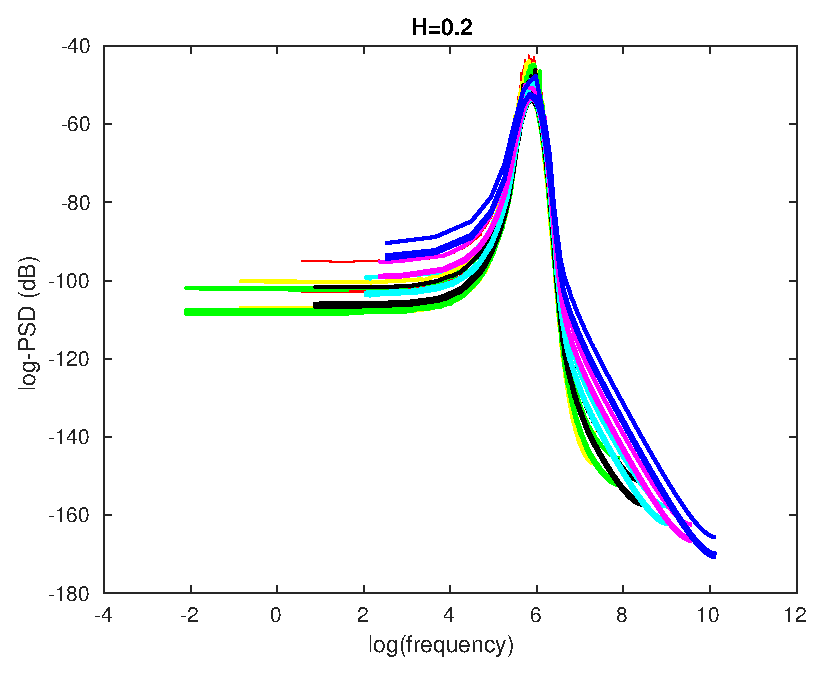
\includegraphics[scale=0.27]{SPEC_Norm_NDel_8_H_2.eps}&
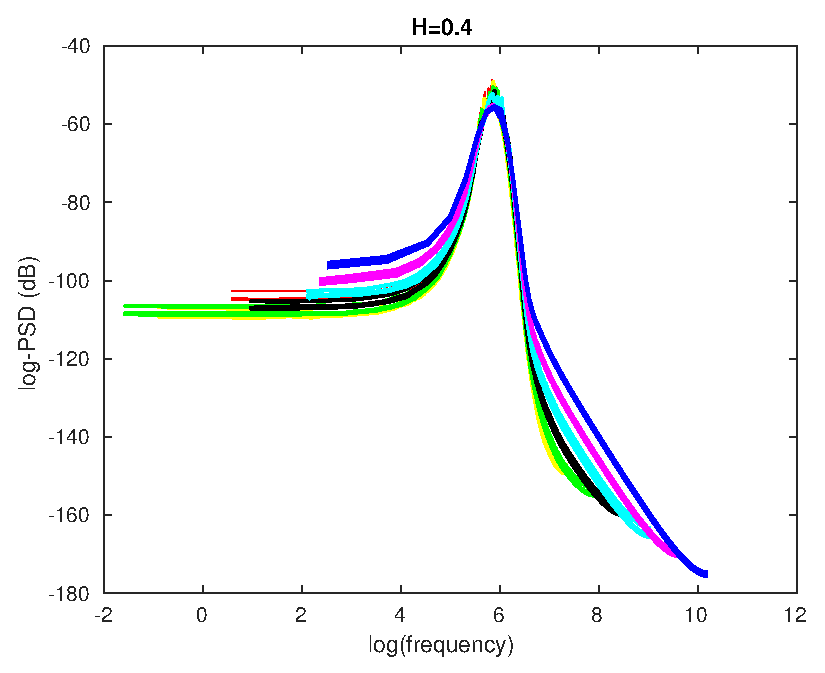
\includegraphics[scale=0.27]{SPEC_Norm_NDel_8_H_4.eps}&
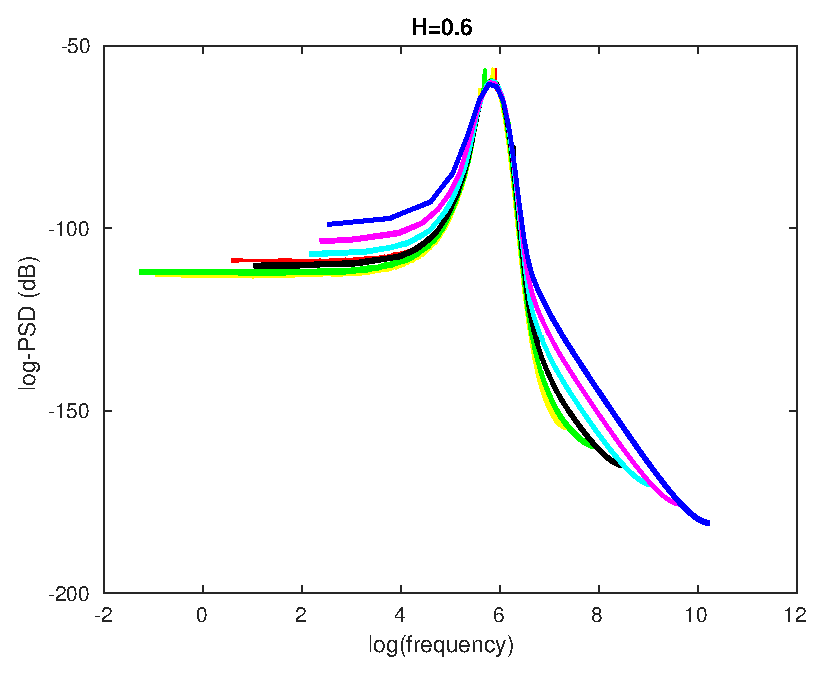
\includegraphics[scale=0.27]{SPEC_Norm_NDel_8_H_6.eps}&
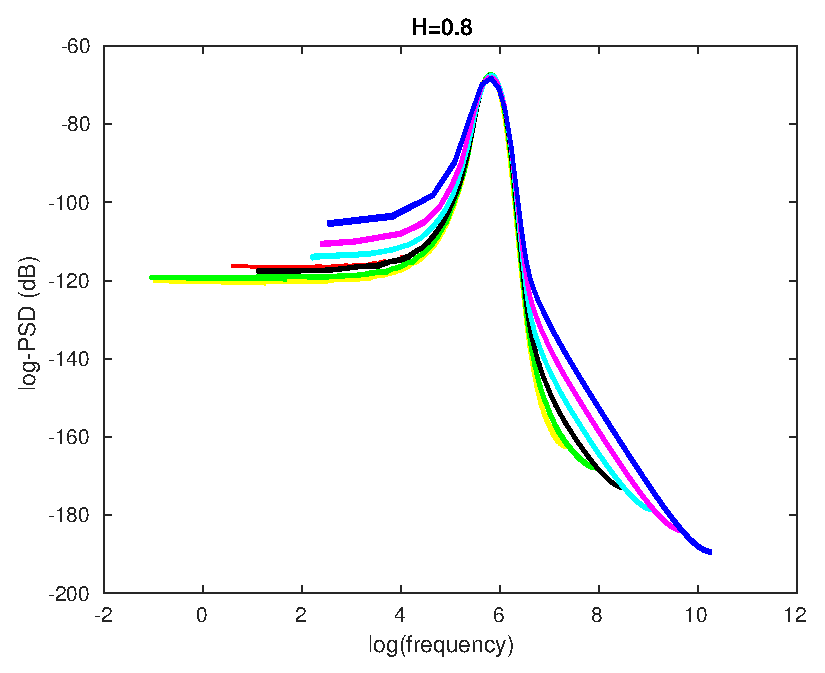
\includegraphics[scale=0.27]{SPEC_Norm_NDel_8_H_8.eps}\\
 $\rho=0.8,~H=0.2$ & $\rho=0.8,~H=0.4$ & $\rho=0.8,~H=0.6$ & $\rho=0.8,~H=0.8$\\
\end{tabular}
\caption{The normalized power spectra of IMFs as a function of $\log_2(f)$, for $H \in \{0.2,0.4, 0.6, 0.8\}$ and $\rho \in \{0, 0.2,0.5,0.8\}$. Overlapping of the frequency bands is obtained using~(\ref{eq: S_k_rho}).}
\label{fig:Normalized_Power_Spectra_MEMD}
\end{figure}

\subsection{Variance distributions}

\begin{figure}[!htbp]
\hspace{-2cm}
\begin{tabular}{c c}
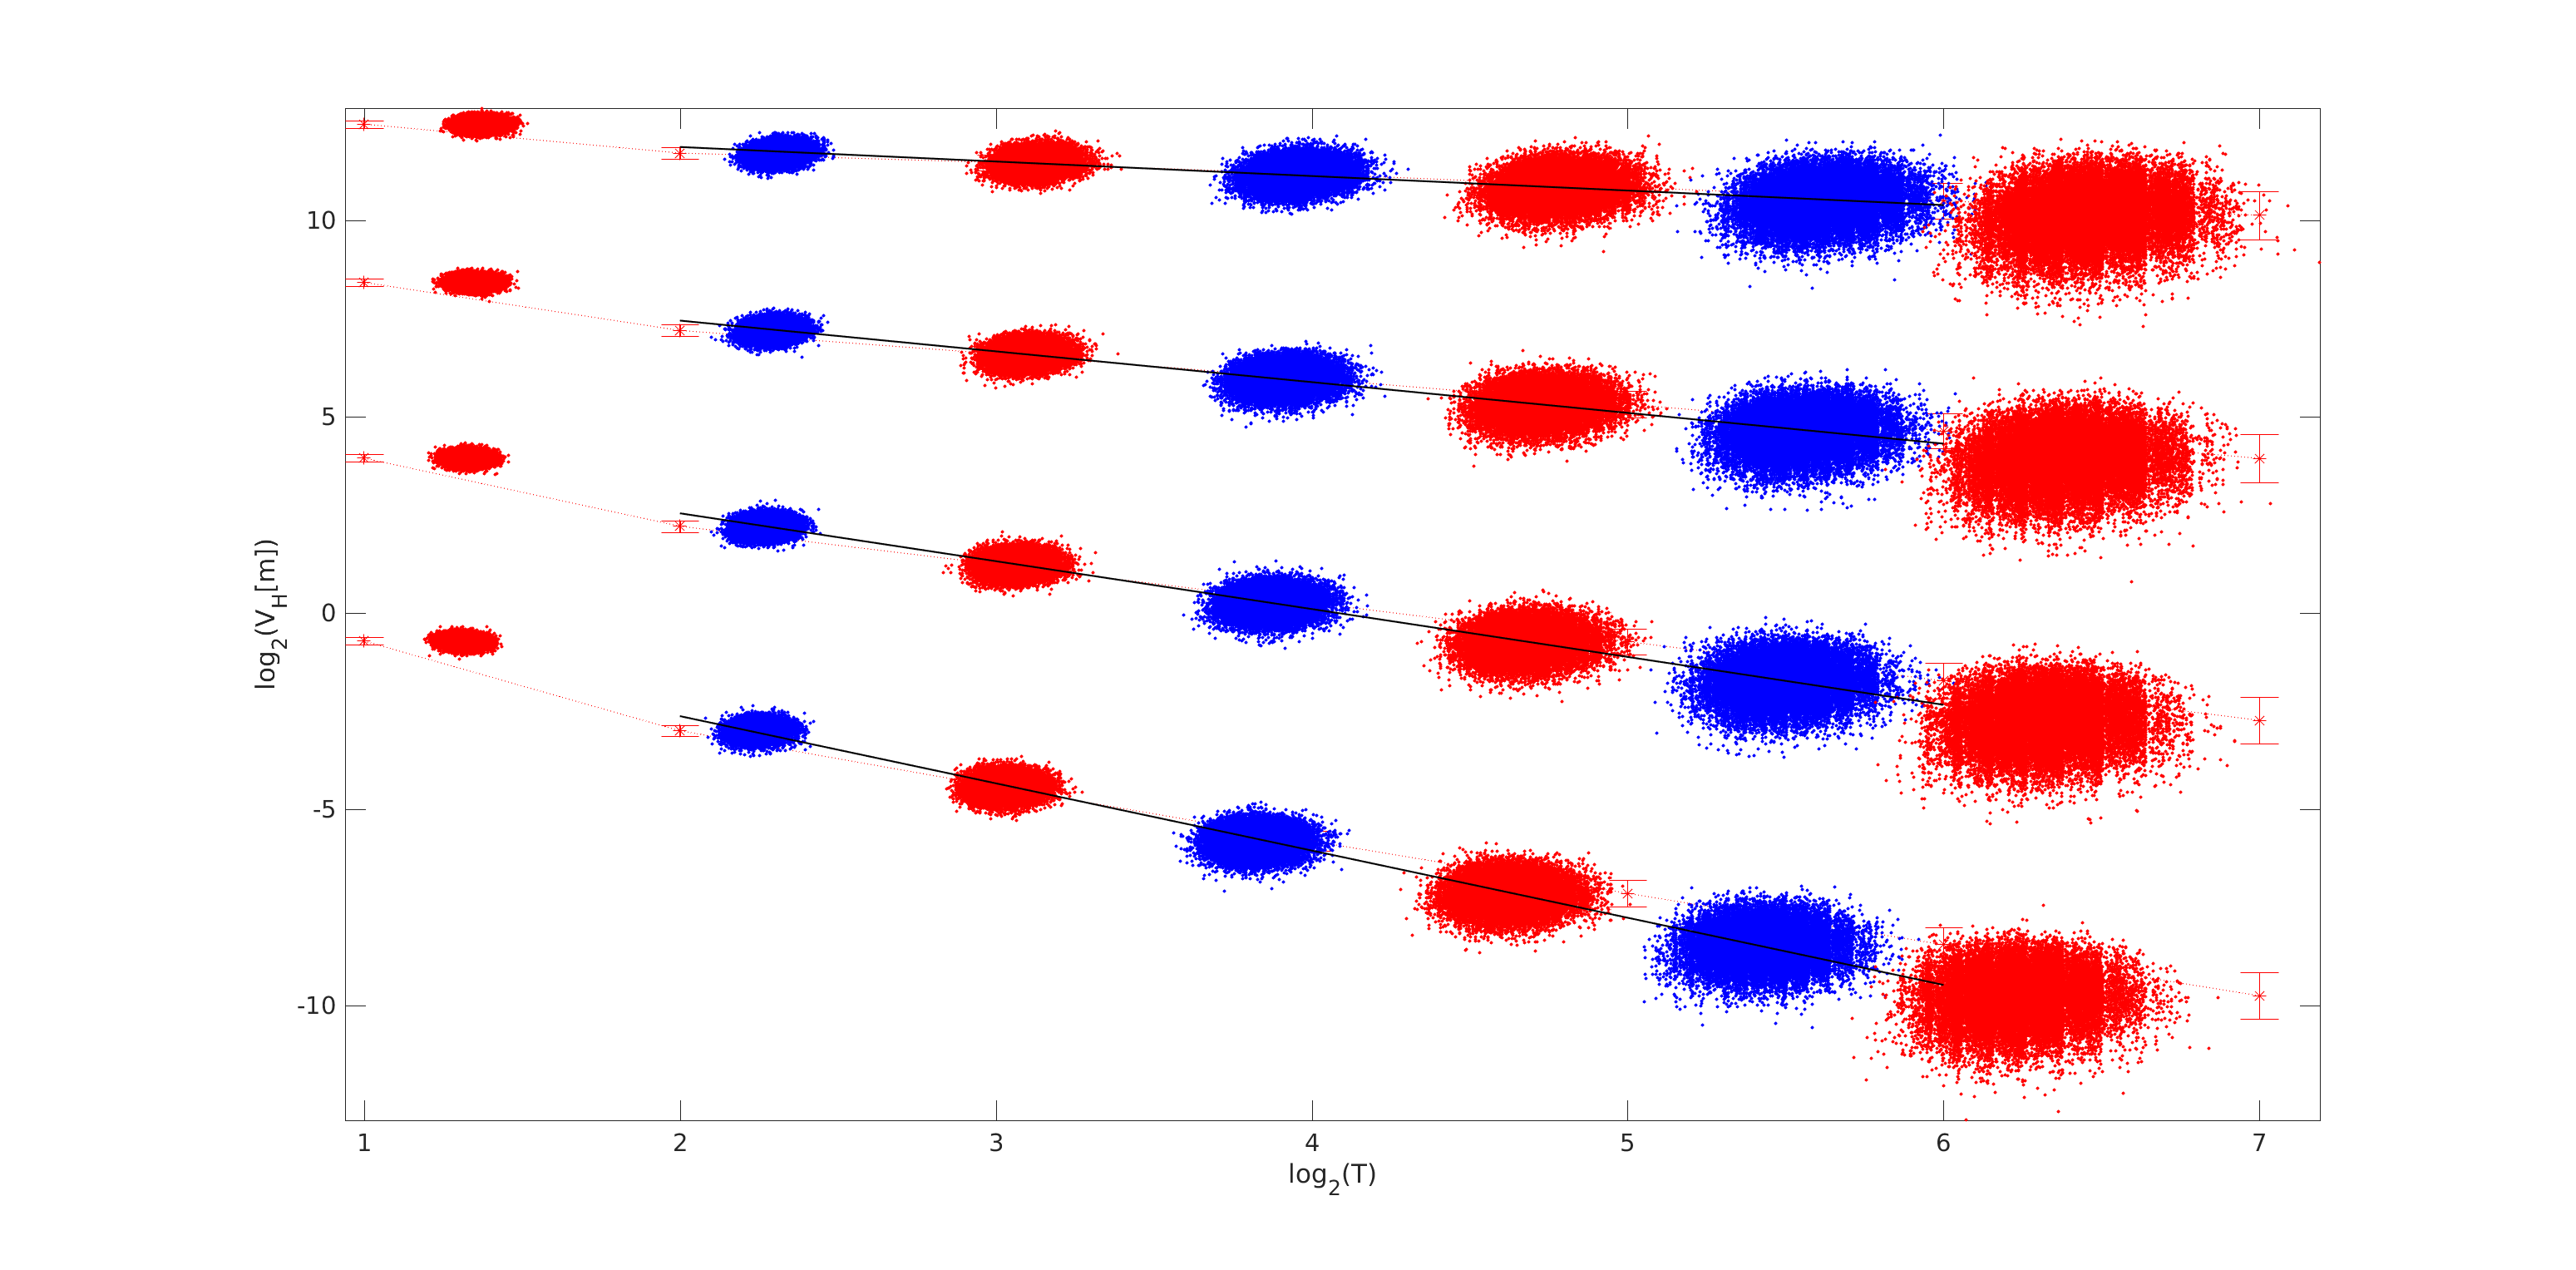
\includegraphics[scale=0.15]{lnE_lnT_MEMD_NDel_0.eps}&
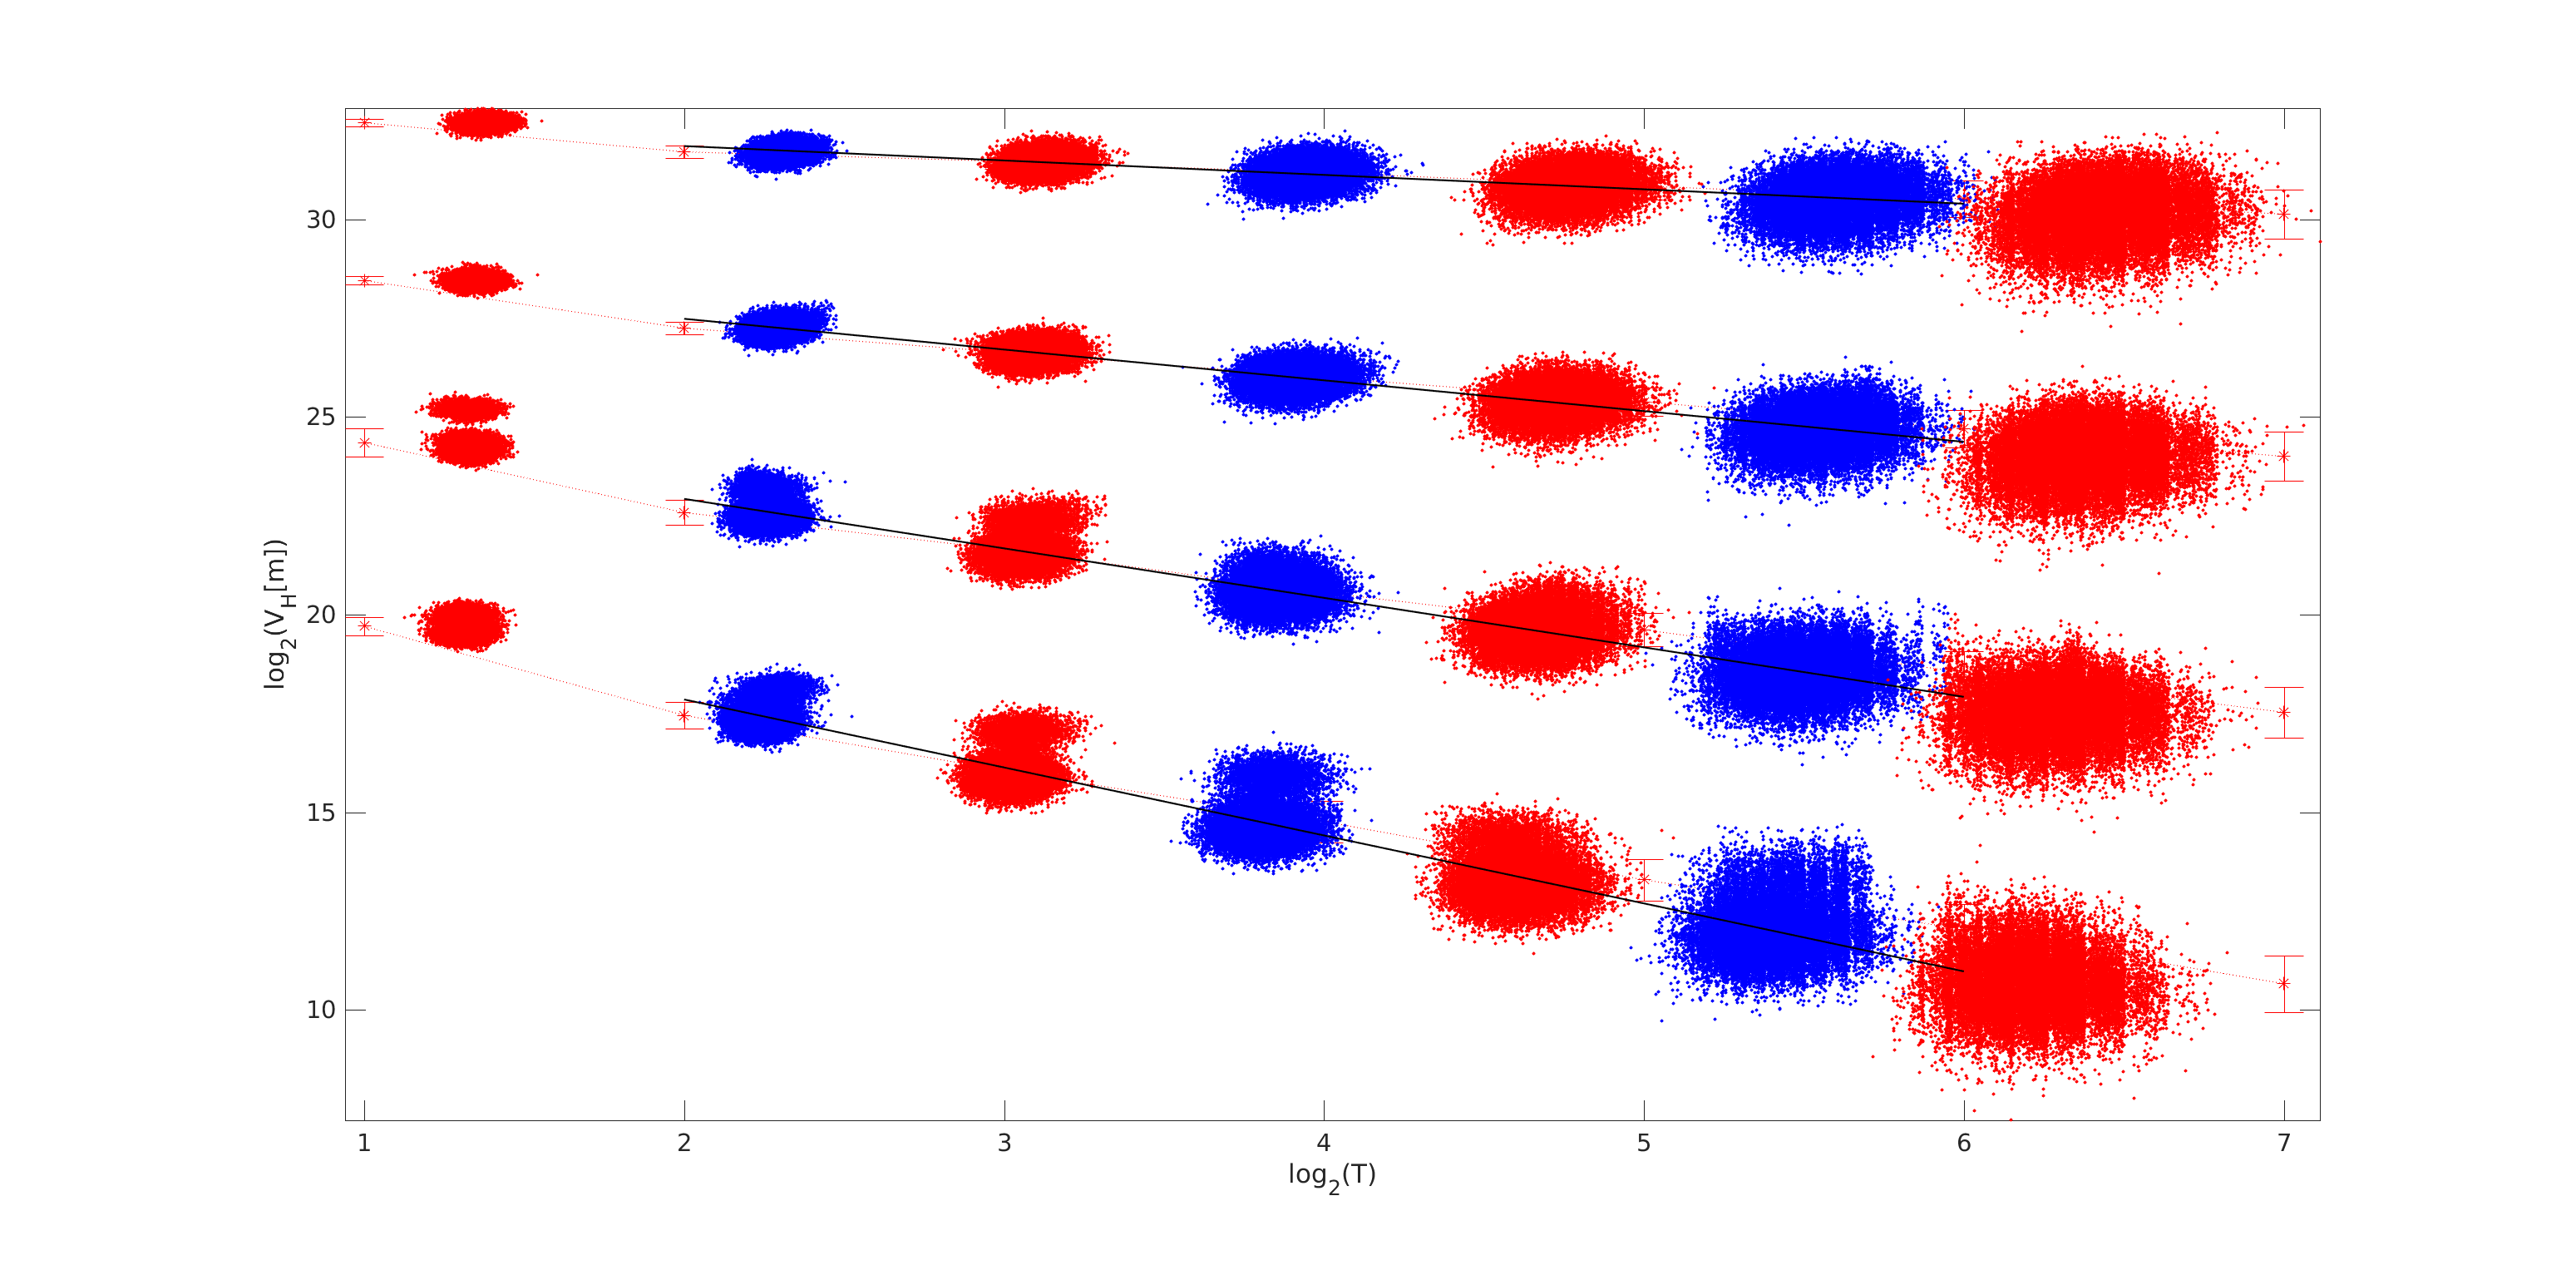
\includegraphics[scale=0.15]{lnE_lnT_MEMD_NDel_2.eps}\\
$\rho=0$ & $\rho=0.2$\\
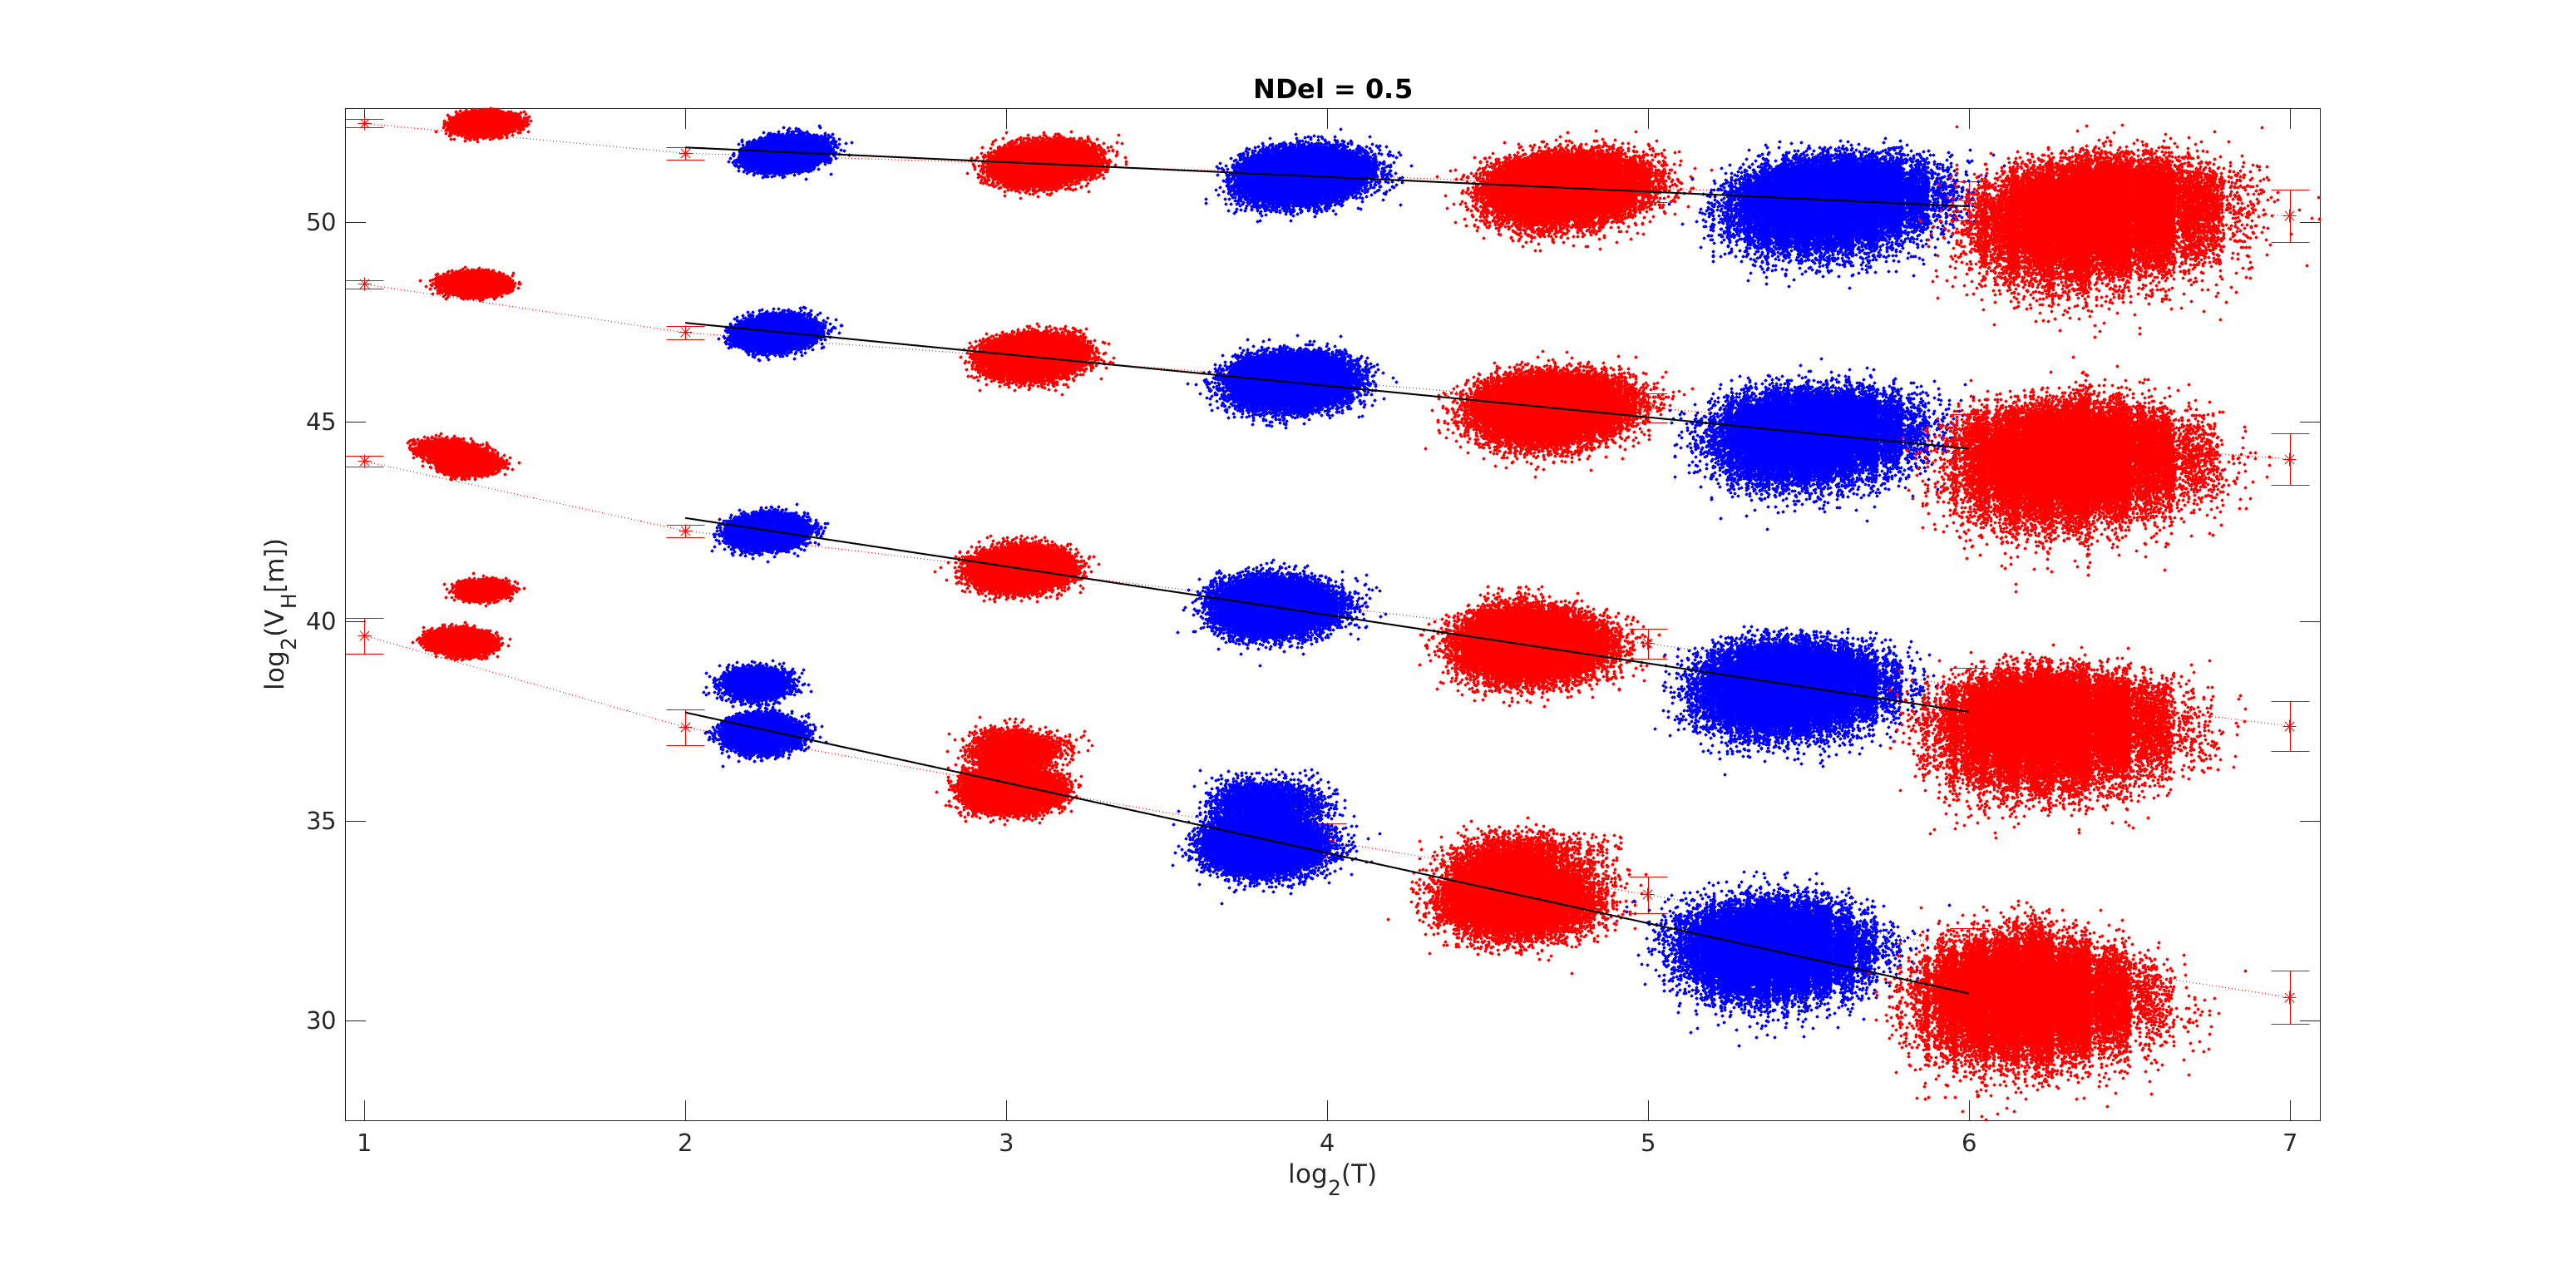
\includegraphics[scale=0.15]{lnE_lnT_MEMD_NDel_5}&
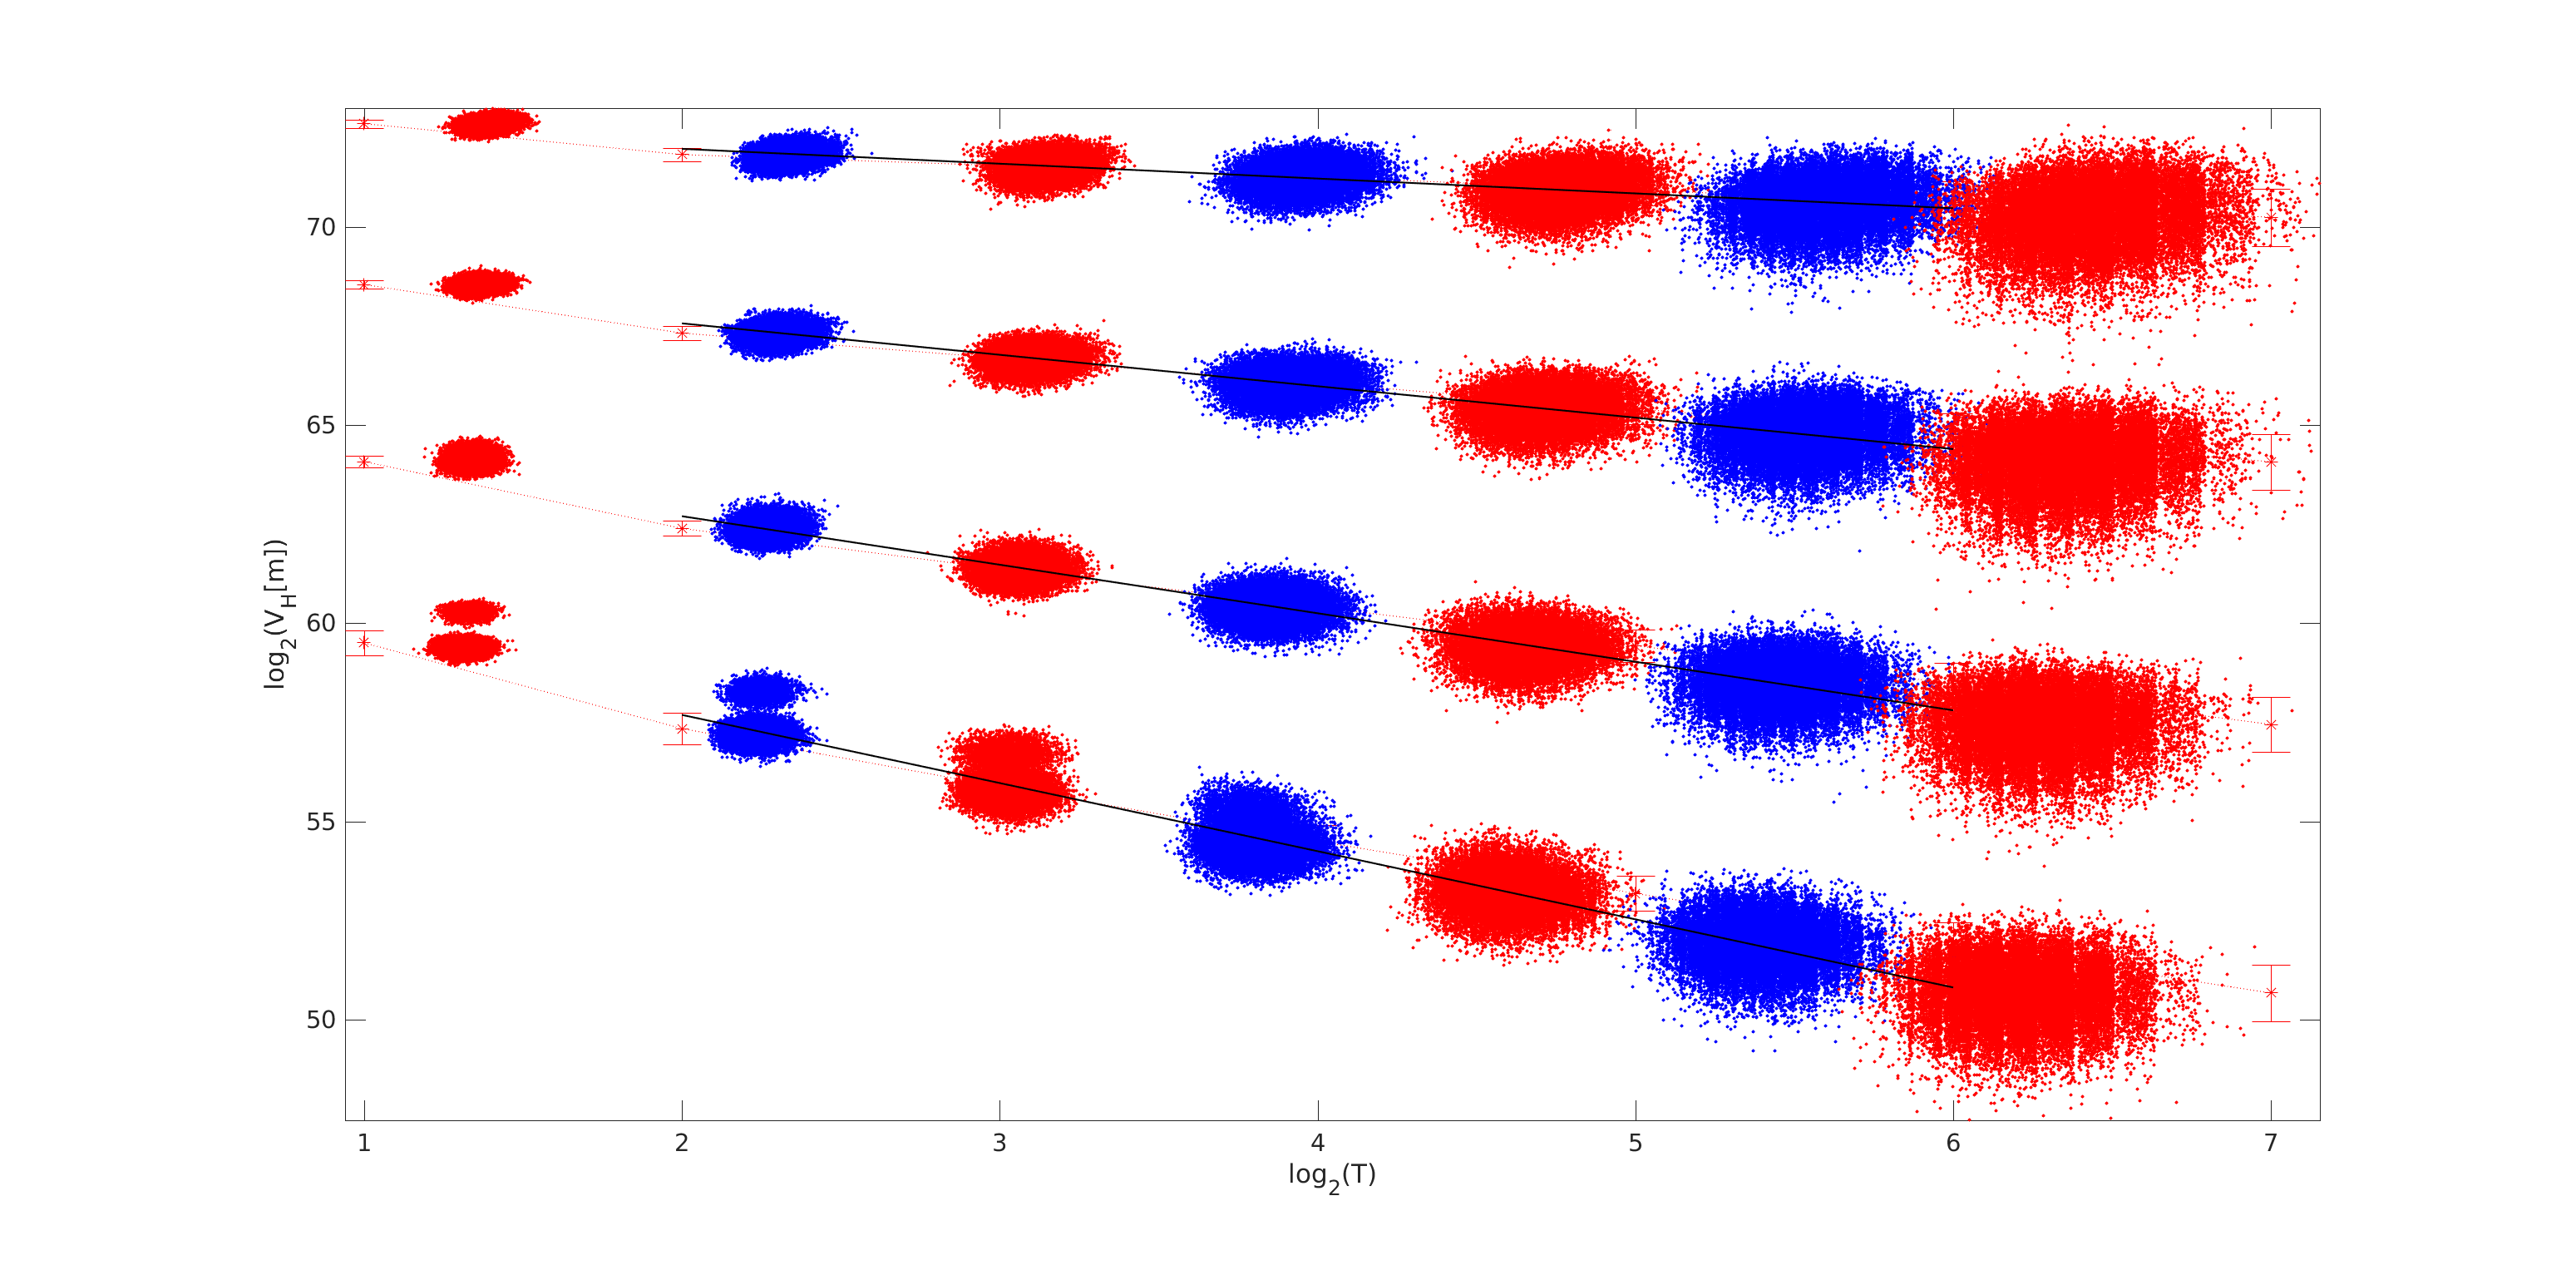
\includegraphics[scale=0.15]{lnE_lnT_MEMD_NDel_8}\\
$\rho=0.5$ & $\rho=0.8$\\
\end{tabular}
\caption[caption]
  {\begin{minipage}[t]{.8\linewidth}Relationship between $V_H[m]$ and $log_2(T)$ for different values of $\rho$.\\The grouped blue and red dots from the upper left to the lower right are the mean energy density (estimation of the variance) as a function of the spectrum-weighted mean period for IMFs $1-7$ over all realizations. The solid black line cutting through the clouds is the weighted linear fit within the IMF indices range $m=2$ to $m=6$. For the sake of clarity, all curves have been shifted upwards to avoid overlapping.\end{minipage}}
\label{fig.logV_logT}
\end{figure}

\begin{figure}[!htbp]
\hspace{-1cm}
\begin{tabular}{c c}
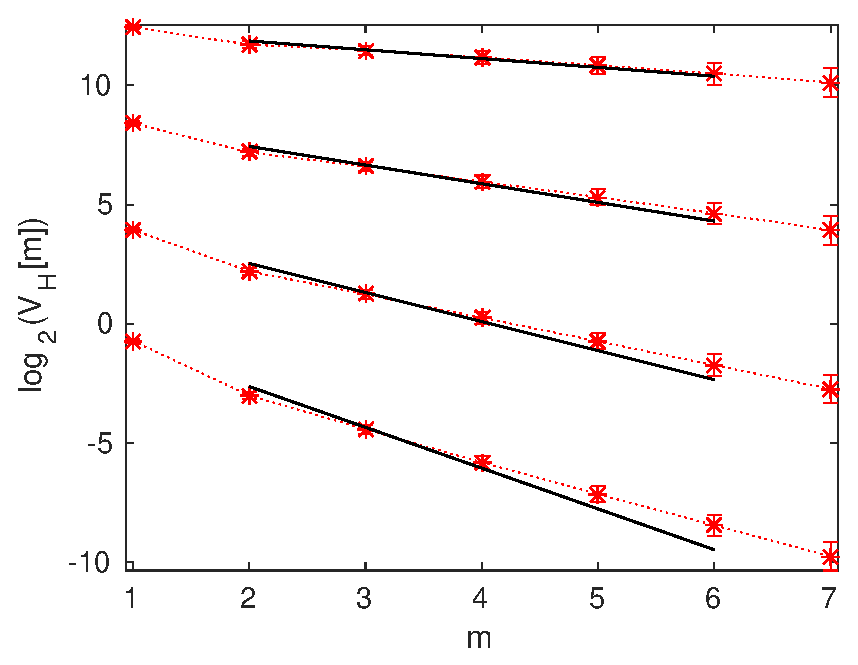
\includegraphics[scale=0.45]{lnE_m_MEMD_NDel_0.eps}&
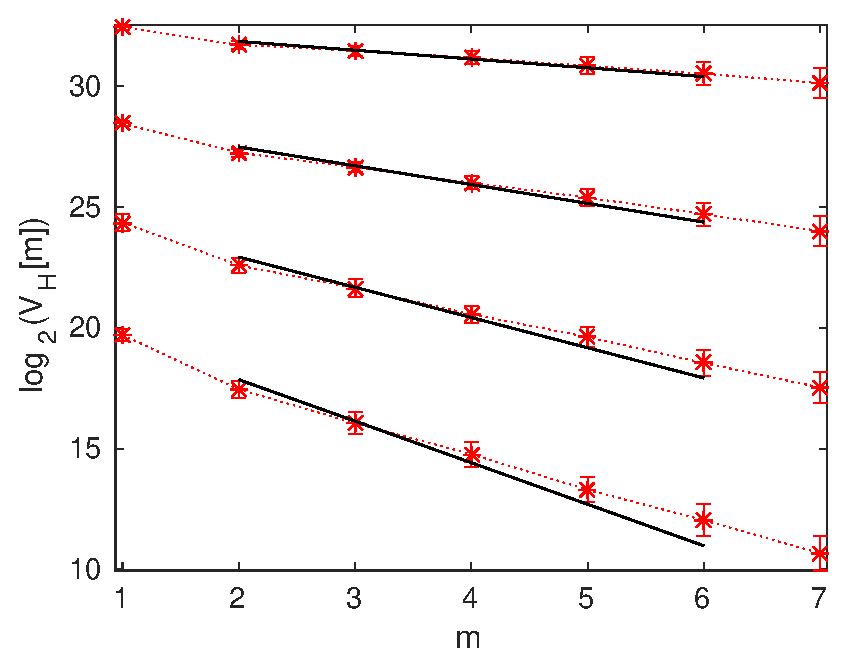
\includegraphics[scale=0.45]{lnE_m_MEMD_NDel_2.eps}\\
$\rho=0$ & $\rho=0.2$\\
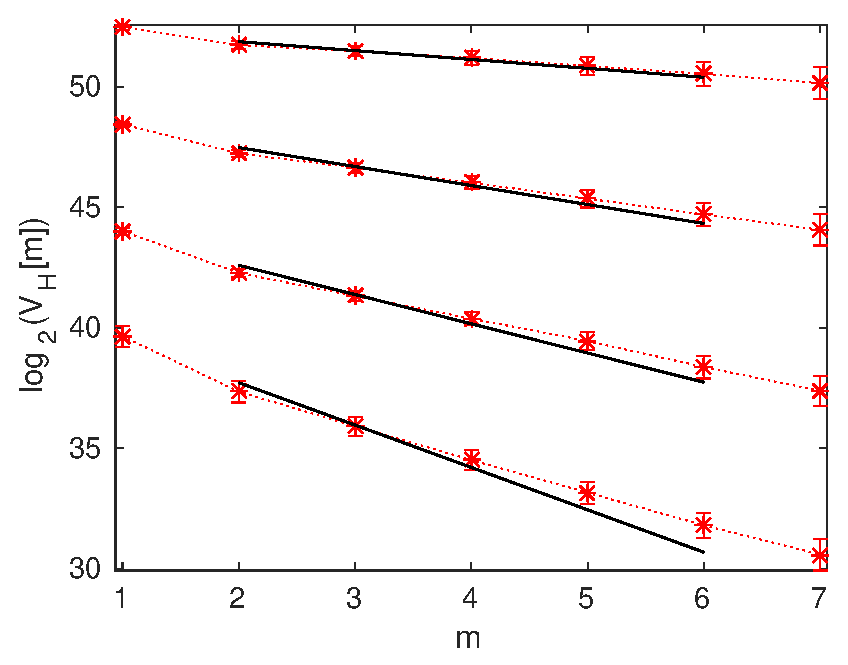
\includegraphics[scale=0.45]{lnE_m_MEMD_NDel_5.eps}&
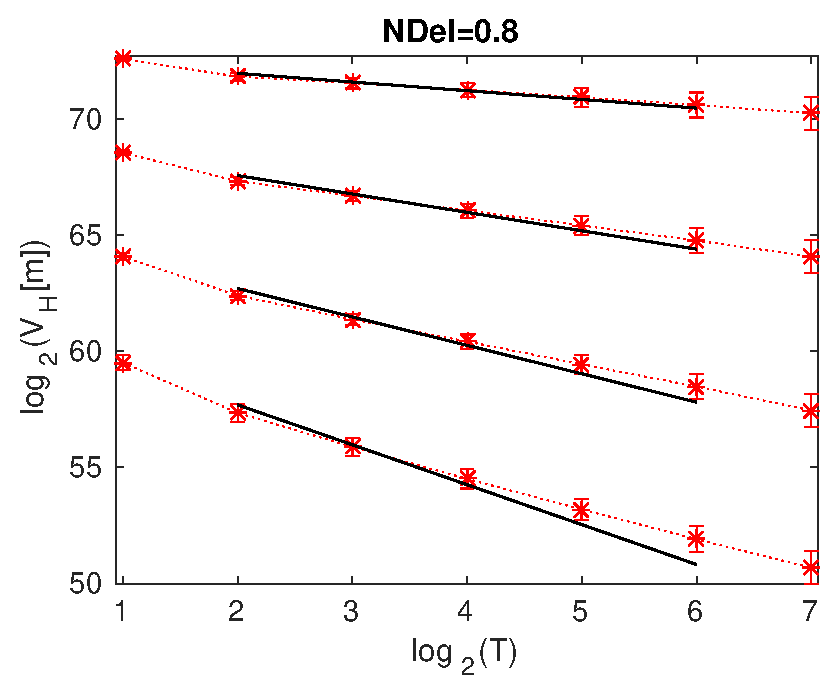
\includegraphics[scale=0.45]{lnE_m_MEMD_NDel_8.eps}\\
$\rho=0.5$ & $\rho=0.8$\\
\end{tabular}
\caption[caption]
  {\begin{minipage}[t]{.8\linewidth} Relationship between $V_H[m]$ and $m$ for different values of $\rho$. The values of the empirical variance estimate are given by red dotted lines for different values of $H$. The error bars correspond to the standard deviation associated with the realizations. The black thin line is the weighted linear fit within the IMF indices range $m=2$ to $m=6$.\\($^{\tiny \dagger}$) scale alignment is almost satisfied, it is highly dependent on the $p$-dimensional envelopes of the original signal. However, in NA-MEMD, the scale misalignment is reduced.\end{minipage}}
\label{fig.logV_logT}
\end{figure}


\section{Correlograms}
We choose to compare all the channels corresponding to the $n^{th}$ IMF. We report in figures~\ref{Fig:Corelation0}, \ref{Fig:Corelation2}, \ref{Fig:Corelation5}, \ref{Fig:Corelation8} alignment results. These figures shows the inter-channel correlations, that is, the correlation matrix $Corr$. $Corr$ is the correlation matrix between $IMF_i^1,  IMF_i^2, \ldots, IMF_i^P$, where $i \in {1, 2, ..., N}$ is the IMF index and $P$ is the number of channels
% RHO is of size p x p x n, where p is the nb of channels and n is th nb of
% imfs. What do represent RHO is the following:
%  RHO is the correlation matrix between I_i_1, I_i_2, ...,I_i_p
%  where i \in {1, 2, ..., n} and I stands for IMF
%  The result of this correlation for the 4^{th} IMF will be as follows:
%            I_4_1   I_4_2   I_4_3   I_4_4   I_4_5 ...ect
% I_4_1        1       v       v       v       v
% I_4_2        v       1       v       v       v
% I_4_3        v       v       1       v       v
% I_4_4        v       v       v       1       v
% I_4_5        v       v       v       v       1
%   .          .       .       .       .       .
%   .          .       .       .       .       .
%   .          .       .       .       .       .
%  etc        etc     etc     etc     etc     etc
%  
\[
Corr_{H,\rho} = 
 \begin{pmatrix}
  1 		& 	c_i^{1,2}	 & 	\cdots	  & 	c_i^{1,P} \\
  c_i^{1,2} &      1		 &  \cdots    &     c_i^{2,P} \\
  \vdots    &      \vdots    &  \ddots    &    \vdots    \\
  c_i^{P,1} &   c_i^{P,2}	 &  \cdots    &      1 \\
 \end{pmatrix}  
\]
Where $c_i^{p,l}$ is correlation coefficient between $IMF_i^p$ and $IMF_i^l$. In other words, it is the correlation coefficient between the $i^{th}$ IMF of channel $p$ and the same $i^{th}$ IMF of channel $l$. So $Corr_{H,\rho} $ is a measure of inter-channel correlation.\\
We notice that when the correlation parameter $\rho$ is different from zero, the correlation between channels is seen clearly, therefore MEMD conserves the inter-channel correlation of the mfGn process.


\begin{figure}[htbp]
  \hspace{-2cm}
  \scalebox{0.85}{\begin{tabular}{c c}
\includegraphics[scale=0.25]{Correlogram_MEMD_NDel_0_H_2.eps}& \hspace{1.2cm}
\includegraphics[scale=0.25]{Correlogram_MEMD_NDel_0_H_4.eps}\\
$\rho=0,~H=0.2$ & $\rho=0,~H=0.4$ \vspace{1cm}\\
\includegraphics[scale=0.25]{Correlogram_MEMD_NDel_0_H_6.eps}& \hspace{1.2cm}
\includegraphics[scale=0.25]{Correlogram_MEMD_NDel_0_H_8.eps}\\
$\rho=0,~H=0.6$ & $\rho=0,~H=0.8$\\
\end{tabular}}
 \caption{Cross-correlations of IMFs for different values of parameters $(\rho, H) \in \{(0,0.2), (0,0.4), (0,0.6), (0,0.8)\}$.}
  \label{Fig:Corelation0}
\end{figure}

\begin{figure}[htbp]
  \hspace{-2cm}
  \scalebox{0.85}{\begin{tabular}{c c}
\includegraphics[scale=0.25]{Correlogram_MEMD_NDel_2_H_2.eps}& \hspace{1.2cm}
\includegraphics[scale=0.25]{Correlogram_MEMD_NDel_2_H_4.eps}\\
$\rho=0,~H=0.2$ & $\rho=0,~H=0.4$ \vspace{1cm}\\
\includegraphics[scale=0.25]{Correlogram_MEMD_NDel_2_H_6.eps}& \hspace{1.2cm}
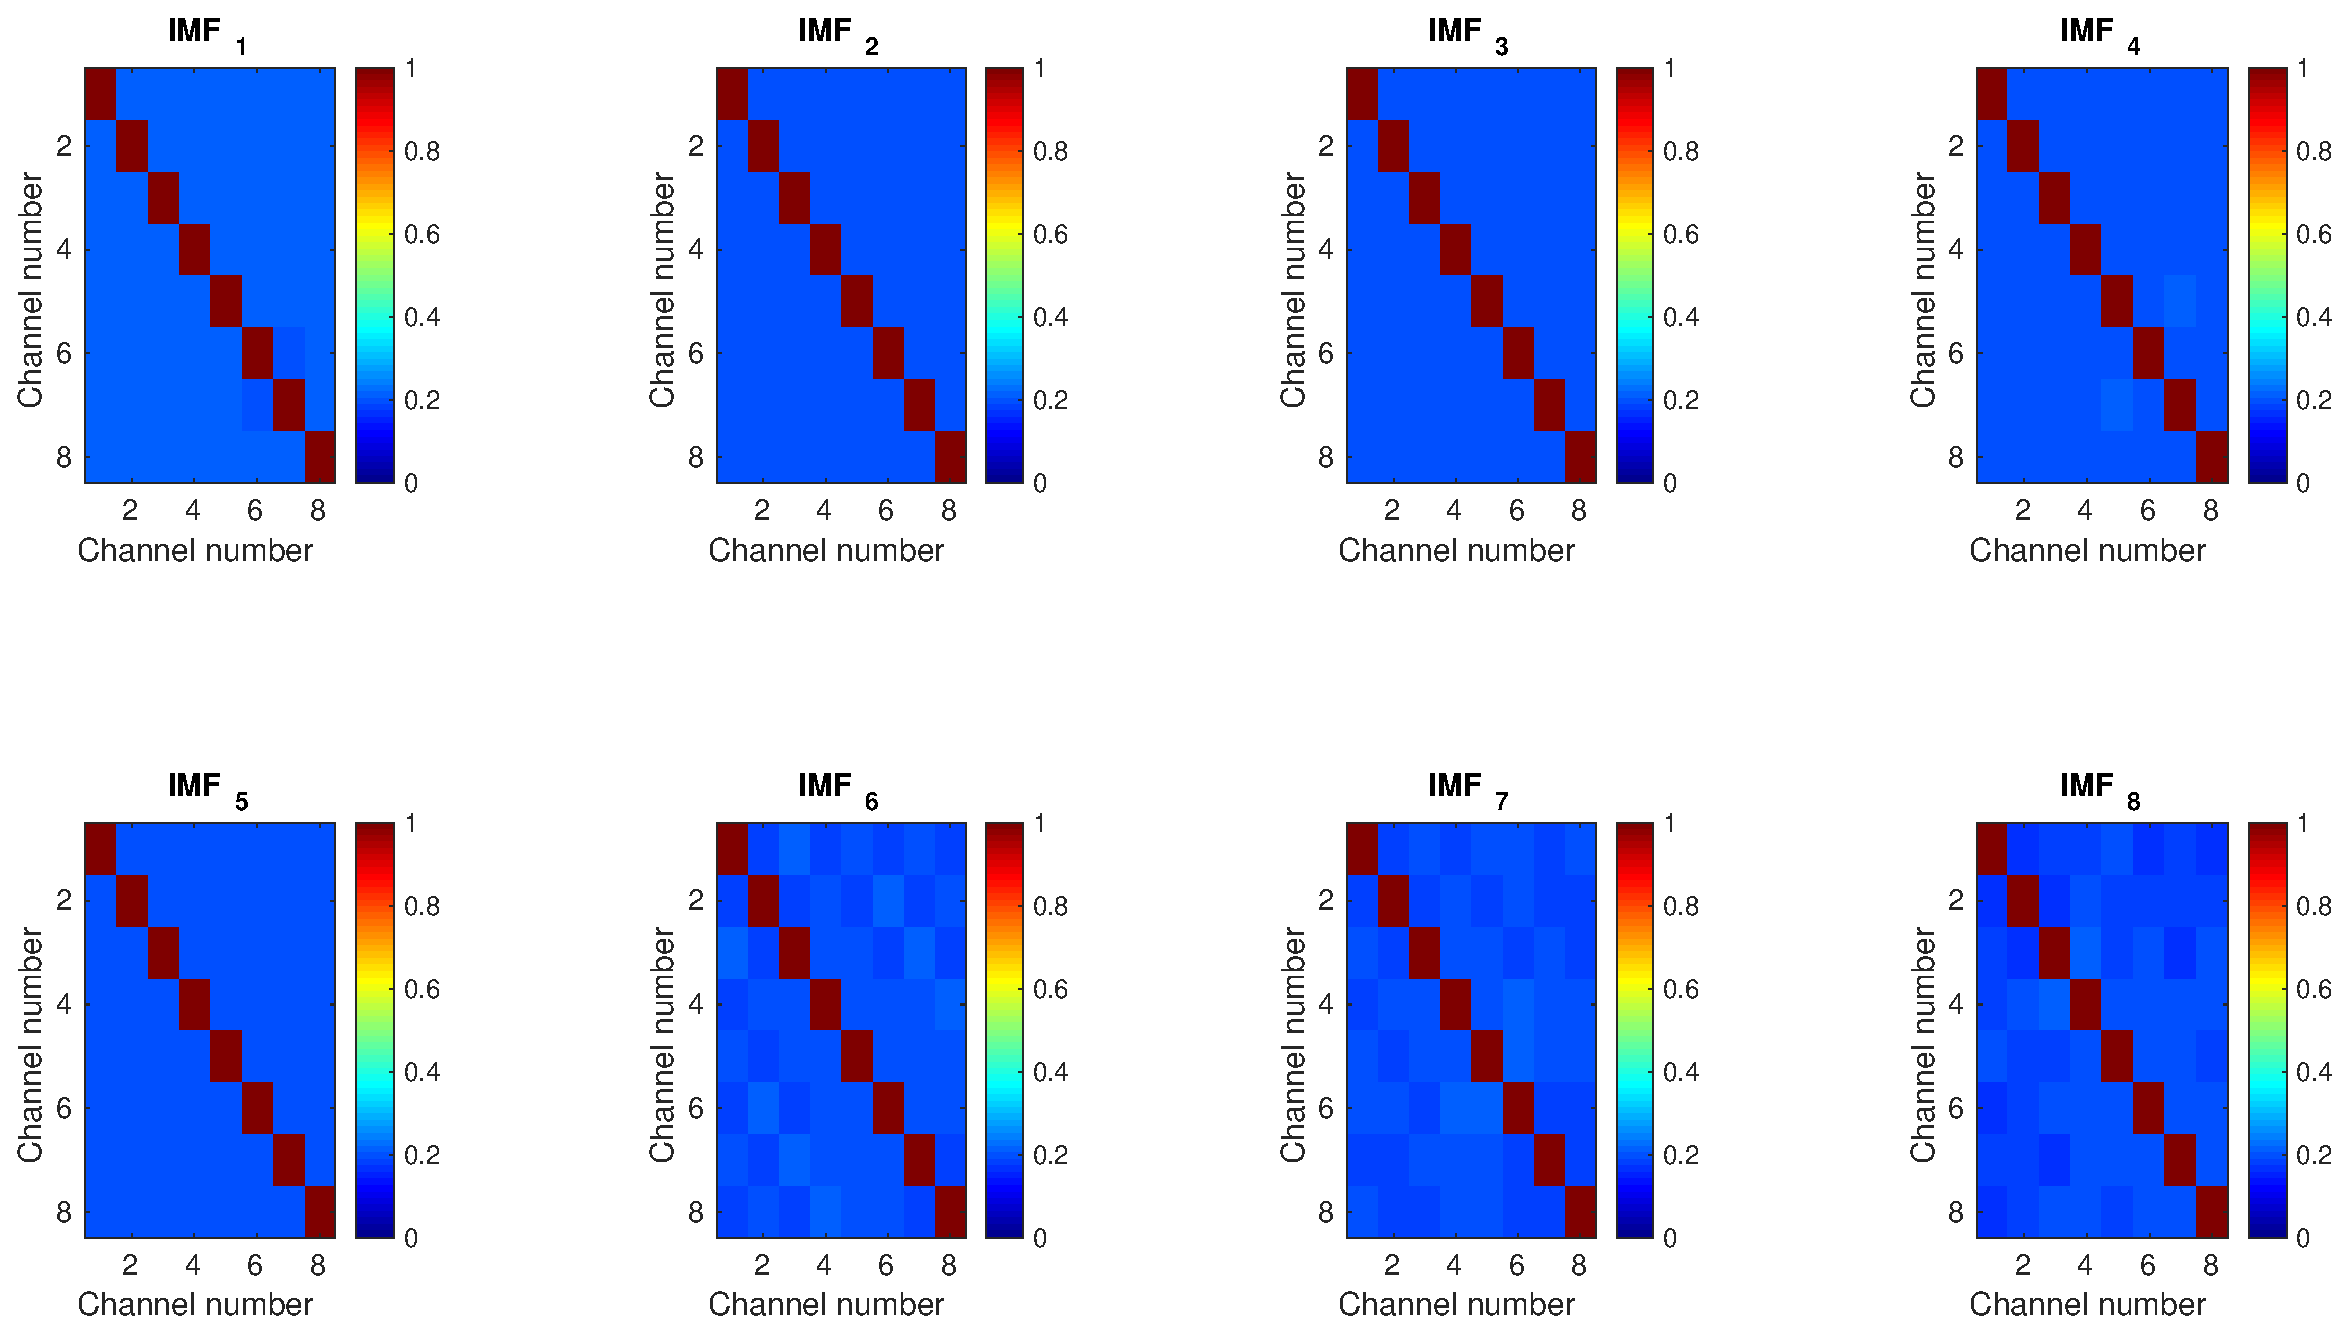
\includegraphics[scale=0.25]{Correlogram_MEMD_NDel_2_H_8.eps}\\
$\rho=0,~H=0.6$ & $\rho=0,~H=0.8$\\
\end{tabular}}
 \caption{Cross-correlations of IMFs for different values of parameters $(\rho, H) \in \{(0.2,0.2), (0.2,0.4), (0.2,0.6), (0.2,0.8)\}$.}
  \label{Fig:Corelation2}
\end{figure}


\begin{figure}[htbp]
  \hspace{-2cm}
  \scalebox{0.85}{\begin{tabular}{c c}
\includegraphics[scale=0.25]{Correlogram_MEMD_NDel_5_H_2.eps}& \hspace{1.2cm}
\includegraphics[scale=0.25]{Correlogram_MEMD_NDel_5_H_4.eps}\\
$\rho=0,~H=0.2$ & $\rho=0,~H=0.4$ \vspace{1cm}\\
\includegraphics[scale=0.25]{Correlogram_MEMD_NDel_5_H_6.eps}& \hspace{1.2cm}
\includegraphics[scale=0.25]{Correlogram_MEMD_NDel_5_H_8.eps}\\
$\rho=0,~H=0.6$ & $\rho=0,~H=0.8$\\
\end{tabular}}
 \caption{Cross-correlations of IMFs for different values of parameters $(\rho, H) \in \{(0.5,0.2), (0.5,0.4), (0.5,0.6), (0.5,0.8)\}$.}
  \label{Fig:Corelation5}
\end{figure}


\begin{figure}[htbp]
  \hspace{-2cm}
  \scalebox{0.85}{\begin{tabular}{c c}
\includegraphics[scale=0.25]{Correlogram_MEMD_NDel_8_H_2.eps}& \hspace{1.2cm}
\includegraphics[scale=0.25]{Correlogram_MEMD_NDel_8_H_4.eps}\\
$\rho=0,~H=0.2$ & $\rho=0,~H=0.4$ \vspace{1cm}\\
\includegraphics[scale=0.25]{Correlogram_MEMD_NDel_8_H_6.eps}& \hspace{1.2cm}
\includegraphics[scale=0.25]{Correlogram_MEMD_NDel_8_H_8.eps}\\
$\rho=0,~H=0.6$ & $\rho=0,~H=0.8$\\
\end{tabular}}
 \caption{Cross-correlations of IMFs for different values of parameters $(\rho, H) \in \{(0.8,0.2), (0.8,0.4), (0.8,0.6), (0.8,0.8)\}$.}
  \label{Fig:Corelation8}
\end{figure}



%----------------------------------------------------------------------------------------
%	BIBLIOGRAPHY
%----------------------------------------------------------------------------------------

\begin{thebibliography}{9}
\bibitem{Amblard2010} 
J. F. Coeurjolly, P. O. Amblard and S. Achard 
\textit{On multivariate fractional brownian motion and multivariate fractional Gaussian noise}. 
 Signal Processing Conference, 2010 18th European, Aalborg, 2010, pp. 1567-1571.

\bibitem{Rehman2011} 
N. ur Rehman and D. P. Mandic, 
\textit{Filter Bank Property of Multivariate Empirical Mode Decomposition}. 
 in IEEE Transactions on Signal Processing, vol. 59, no. 5, pp. 2421-2426, May 2011.

\end{thebibliography}

\end{document}